\documentclass[10pt,letterpaper]{article}
\usepackage[T1]{fontenc}
\usepackage{lmodern,microtype}
\usepackage[margin=0.72in,top=0.69in,bottom=0.73in,columnsep=0.25in]{geometry}
\usepackage{amsmath,amssymb,amsthm,mathtools,mathrsfs,bm}
\usepackage{booktabs,array,tabularx,longtable,multirow,enumitem}
\usepackage{tikz}
\usetikzlibrary{arrows.meta,positioning,calc,fit,backgrounds,decorations.pathreplacing}
\usepackage{algorithm}
\usepackage[noend]{algpseudocode}
\usepackage{listings,xurl,xcolor,caption,subcaption,float}
\usepackage[numbers,sort&compress]{natbib}
\usepackage[hypertexnames=false,colorlinks=true,linkcolor=blue!40!black,citecolor=blue!40!black,urlcolor=blue!40!black]{hyperref}
\usepackage[nameinlink,noabbrev]{cleveref}
\usepackage{fancyhdr}
\definecolor{deepblue}{RGB}{26,64,91}
\definecolor{softblue}{RGB}{237,244,247}
\definecolor{softgray}{RGB}{246,247,249}
\definecolor{softred}{RGB}{250,239,234}
\definecolor{forest}{RGB}{32,103,86}
\definecolor{rust}{RGB}{155,65,40}
\newtheorem{theorem}{Theorem}
\newtheorem{proposition}[theorem]{Proposition}
\newtheorem{lemma}[theorem]{Lemma}
\newtheorem{corollary}[theorem]{Corollary}
\newtheorem{definition}[theorem]{Definition}
\newtheorem{remark}[theorem]{Remark}
\newtheorem{example}[theorem]{Example}
\newtheorem{claim}[theorem]{Claim}
\newcommand{\Aalg}{\mathcal A}
\newcommand{\Ffam}{\mathcal F}
\newcommand{\Zalg}{\mathcal Z}
\newcommand{\Xfib}{\mathcal X}
\newcommand{\FF}{\mathbb F_2}
\newcommand{\one}{\mathbf 1}
\newcommand{\ee}{\mathbf e}
\newcommand{\rank}{\operatorname{rank}}
\newcommand{\nullity}{\operatorname{nullity}}
\newcommand{\offdiag}{\operatorname{offdiag}}
\newcommand{\supp}{\operatorname{supp}}
\newcommand{\Span}{\operatorname{span}}
\newcommand{\Sink}{\operatorname{Sink}}
\newcommand{\im}{\operatorname{im}}
\newcommand{\rad}{\operatorname{rad}}
\newcommand{\diag}{\operatorname{diag}}
\newcommand{\cA}{\mathsf A}
\newcommand{\QD}{Q}
\newcommand{\ketbra}[2]{|#1\rangle\!\langle#2|}
\newcommand{\code}[1]{\nolinkurl{#1}}
\DeclareMathOperator{\coacc}{coacc}
\DeclareMathOperator{\wt}{wt}
\setlist[itemize]{leftmargin=1.4em,itemsep=0.15em,topsep=0.3em}
\setlist[enumerate]{leftmargin=1.7em,itemsep=0.15em,topsep=0.3em}
\captionsetup{font=small,labelfont=bf,labelsep=period}
\lstset{basicstyle=\ttfamily\footnotesize,backgroundcolor=\color{softgray},frame=single,
 rulecolor=\color{black!15},breaklines=true,columns=fullflexible,keepspaces=true,showstringspaces=false}
\newenvironment{proofbox}{\begin{center}\begin{minipage}{0.94\linewidth}\hrule\vspace{0.5em}}{\vspace{0.4em}\hrule\end{minipage}\end{center}}
\pagestyle{fancy}\fancyhf{}\fancyfoot[C]{\small\thepage}\renewcommand{\headrulewidth}{0pt}
\setlength{\parindent}{1em}
\setlength{\emergencystretch}{1.3em}
\hypersetup{pdftitle={Forbidden heaps and the spectral solution of free-fermion-in-disguise circuits},pdfauthor={Istvan Vona},pdfsubject={Canonical transfer-matrix classification; exact certificates and a sector-aware polynomial-root solution}}
\author{Istvan Vona}
\date{10 November 2026}
\newcommand{\hgraph}[2]{%
 \begin{scope}[shift={(#1)},scale=#2]
 \foreach \v/\x/\y in {A/0/0,B/0.85/0,C/1.65/0.65,D/1.65/-0.65,E/2.45/0,F/3.3/0}
 {\node[circle,draw=deepblue,fill=white,inner sep=0pt,minimum size=4.6mm,font=\scriptsize] (\v) at (\x,\y) {\v};}
 \end{scope}}
\begin{document}
\twocolumn[\begin{@twocolumnfalse}
\begin{center}
{\LARGE\bfseries Forbidden heaps and the spectral solution\\[0.17em]of free-fermion-in-disguise circuits}\par
\vspace{0.7em}
{\large Istvan Vona}\par
\vspace{0.3em}
{\normalsize 10 November 2026}\par
\vspace{0.7em}
\begin{minipage}{0.94\textwidth}\small
\textbf{Abstract.} The spectrum of a free-fermion-in-disguise (FFD) circuit can depend on the order of its gates, even when every local gate is unchanged. We classify the open, one-pass palindromic circuits whose canonical transfer polynomial has commuting coefficients and central inversion. Commuting gate exchanges reduce a permutation to a heap: the relative order of every noncommuting pair. The criterion is local. A heap is admissible precisely when it avoids twenty orientations of a single six-vertex graph, or five patterns up to reflection and reversal. The transfer polynomial follows directly from the circuit expansion, with a binary-nullity grading that counts temporal overlaps rather than selected gates. Its generic spectrum is obtained from polynomial roots, with central-sector sign constraints stated explicitly. A bounded-frontier algorithm computes the required sector polynomials without constructing the many-body matrices. The all-length proof combines a local obstruction, a triangle-interlacement reduction, and exact finite certificates. Complete proofs, pseudocode, and a reproducible verification record are supplied below. The necessity statement concerns this canonical transfer construction, not every conceivable free-fermion representation.
\end{minipage}
\end{center}\vspace{1.1em}
\end{@twocolumnfalse}]

\paragraph{The ordering problem.}
Free fermions in disguise have a factorized many-body spectrum without an evident Jordan--Wigner reduction of their local spin operators \cite{Fendley2019,ElmanChapmanFlammia2021}. For quantum circuits, free-fermion solvability is sensitive to the arrangement of the gates. Pozsgay and Fukai posed this ordering problem \cite{PozsgayFukai2025}; Sz\'asz-Schagrin, Cristani, Piroli, and Vernier subsequently constructed transfer matrices and polynomial-root solutions for three staircase and brickwork families, conventionally called I, II, and III \cite{SzaszSchagrinEtAl2026}.

Here we treat an arbitrary permutation within a fixed class of palindromes. The result has two parts: a finite forbidden-pattern criterion for the canonical transfer family, and an explicit spectral solution for every accepted heap. Neither translation invariance nor a repeating circuit architecture is required.

The open FFD algebra is generated by Hermitian involutions satisfying
\begin{equation}\label{L:algebra}
 h_j^2=1,\quad
 h_jh_k=\begin{cases}-h_kh_j,&1\le |j-k|\le2,\\h_kh_j,&|j-k|>2.\end{cases}
\end{equation}
With $u_j=\exp(i\phi_jh_j/2)$ and a permutation $\pi$ of $[M]$, set
\begin{equation}\label{L:circuit}
 G_\pi=u_{\pi_1}\cdots u_{\pi_M},\qquad V_\pi=G_\pi G_\pi^T.
\end{equation}
Here $T$ reverses products and fixes each $h_j$ and the scalar $i$; it is not the adjoint. Thus the second half retraces the first, with the same angles.

\paragraph{A heap forgets only irrelevant ordering.}
Draw an edge between labels at distance one or two, obtaining the graph $F_M=P_M^2$. Direct each edge from the gate appearing earlier in the half-word to the gate appearing later. This acyclic orientation is the \emph{heap} $D$. Its transitive closure is a partial order; its linear extensions are exactly the words related by adjacent exchanges of commuting gates \cite{CartierFoata1969}. All those words give the same circuit. Figure~\ref{L:heapfig} illustrates the distinction between the spatial graph and its temporal ordering.

\begin{figure}[t]
\centering
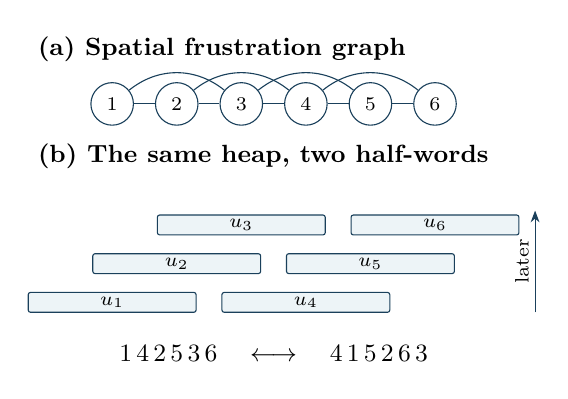
\begin{tikzpicture}[x=0.82cm,y=0.63cm,font=\small]
\node[anchor=west,font=\small\bfseries] at (-0.3,5.1) {(a) Spatial frustration graph};
\foreach \j in {1,...,6}{\node[circle,draw=deepblue,fill=white,minimum size=5.4mm,inner sep=0pt] (n\j) at (\j,4.0) {\scriptsize\j};}
\foreach \j [evaluate=\j as \k using int(\j+1)] in {1,...,5}{\draw[deepblue] (n\j)--(n\k);}
\foreach \j [evaluate=\j as \k using int(\j+2)] in {1,...,4}{\draw[deepblue,bend left=39] (n\j) to (n\k);}
\node[anchor=west,font=\small\bfseries] at (-0.3,2.95) {(b) The same heap, two half-words};
\foreach \j/\t in {1/0,4/0,2/1,5/1,3/2,6/2}{
 \draw[fill=softblue,draw=deepblue,rounded corners=0.8pt] (\j-1.30,\t*0.78-0.20) rectangle (\j+1.30,\t*0.78+0.20);
 \node[font=\scriptsize] at (\j,\t*0.78) {$u_{\j}$};}
\draw[-{Stealth[length=1.5mm]},deepblue] (7.55,-0.20)--(7.55,1.85);
\node[rotate=90,font=\scriptsize,anchor=south] at (7.60,0.83) {later};
\node[align=center,font=\small] at (3.5,-1.03) {$1\,4\,2\,5\,3\,6\quad\longleftrightarrow\quad4\,1\,5\,2\,6\,3$};
\end{tikzpicture}
\caption{\textbf{From a word to a heap.} (a) An edge means anticommutation, not a physical wire. (b) Draw gate $j$ as an interval centered at $j$; overlapping intervals cannot pass through one another. Gates in each displayed row commute. Exchanging them changes the word but not the heap or the palindrome. Vertical position shows the relative order in the half-word, not the direction of operator action on a state.}
\label{L:heapfig}
\end{figure}

\paragraph{The canonical transfer polynomial.}
Write $x_j=\cos\phi_j$ and $y_j=\sin\phi_j$. For a selected set $S$, let $e_D(v,S)$ be the parity of its selected out-neighbors. The set is \emph{feasible} when $e_D(v,S)=0$ at every selected vertex. Peeling the palindrome from its outside gives the exact expansion
\begin{align}
 V_D&=\sum_{S\text{ feasible}}a_D(S)H_D(S),\label{L:expansion}\\
 a_D(S)&=i^{|S|}\prod_{j\in S}y_j
       \prod_{\substack{j\notin S\\e_D(j,S)=0}}x_j,\label{L:amplitude}
\end{align}
where $H_D(S)$ is the product of the selected generators in temporal order.

The nontrivial step is assigning a spectral degree. In temporal coordinates on $S$, let $N_{ab}=1$ when $a<b$ and the corresponding generators anticommute. Work over $\FF$ and define
\begin{equation}\label{L:grade}
 \begin{aligned}
 K_D(S)&=\offdiag[(I+N)^T(I+N)],\\
 \nu_D(S)&=\nullity K_D(S).
 \end{aligned}
\end{equation}
A column of $I+N$ marks an event together with its earlier selected neighbors. Thus $K$ records the pairwise overlaps of these \emph{predecessor footprints}, excluding self-overlap. This is not a gate count: a feasible three-gate temporal fork has $\nu=1$.

The canonical polynomial is
\begin{equation}\label{L:transfer}
 \boxed{\cA_D(z)=\sum_{S\text{ feasible}}a_D(S)z^{\nu_D(S)}H_D(S).}
\end{equation}
It obeys $\cA_D(1)=V_D$, $\cA_D(0)=a_0\one$ with $a_0=\prod_jx_j$, and $\cA_D(z)^\dagger=\cA_D(-z)$ for real $z$.

\paragraph{The local classification.}
The obstruction graph $H$ has two triangles sharing an edge and a pendant edge at each end:
\begin{equation}\label{L:edges}
 E(H)=\{AB,BC,BD,CD,CE,DE,EF\}.
\end{equation}
Its relevant copies occupy
\begin{equation}\label{L:sites}
 (A,B,C,D,E,F)=(a,a+2,a+3,a+4,a+5,a+7).
\end{equation}
Orient the edges by any one of the five words
\begin{equation}\label{L:reps}
 \begin{gathered}
 \texttt{ADBCFE},\quad\texttt{ADBCEF},\quad\texttt{ACBFED},\\
 \texttt{ACBDFE},\quad\texttt{ACBDEF}.
 \end{gathered}
\end{equation}
Reversing every arrow and reflecting $A\leftrightarrow F$, $B\leftrightarrow E$, $C\leftrightarrow D$ produces twenty distinct forbidden orientations (Fig.~\ref{L:badfig}). The other two sites in the eight-site window are ignored, not deleted from the circuit.

\begin{theorem}[Canonical FFD classification]\label{thm:main}\label{L:main}
For every open-chain length and every heap $D$, the following are equivalent: (i) no translated copy in \eqref{L:sites} has a forbidden orientation; (ii) the family \eqref{L:transfer} satisfies
\begin{align}
 \deg\cA_D&\le s_M:=\lceil M/3\rceil,\label{L:degree}\\
 [\cA_D(z),\cA_D(w)]&=0,\label{L:comm}\\
 \cA_D(z)\cA_D(-z)&\in Z(\Aalg_M)[z^2].\label{L:inv}
\end{align}
These are identities for arbitrary angles. Sufficiency is proved by exact finite certificates valid at every length.
\end{theorem}

The criterion takes $O(M)$ comparisons once the positions of the labels in $\pi$ are known. All heaps of lengths $M\le7$ pass. At $M=8$, precisely $1{,}054$ of the $1{,}458$ heaps pass; these are counts of heaps, not permutations. A forbidden heap fails the canonical commutation identity generically, although special angle choices can remove the obstruction. Crucially, this does not exclude a different transfer family or an exceptional free spectrum.

\begin{figure*}[t]
\centering
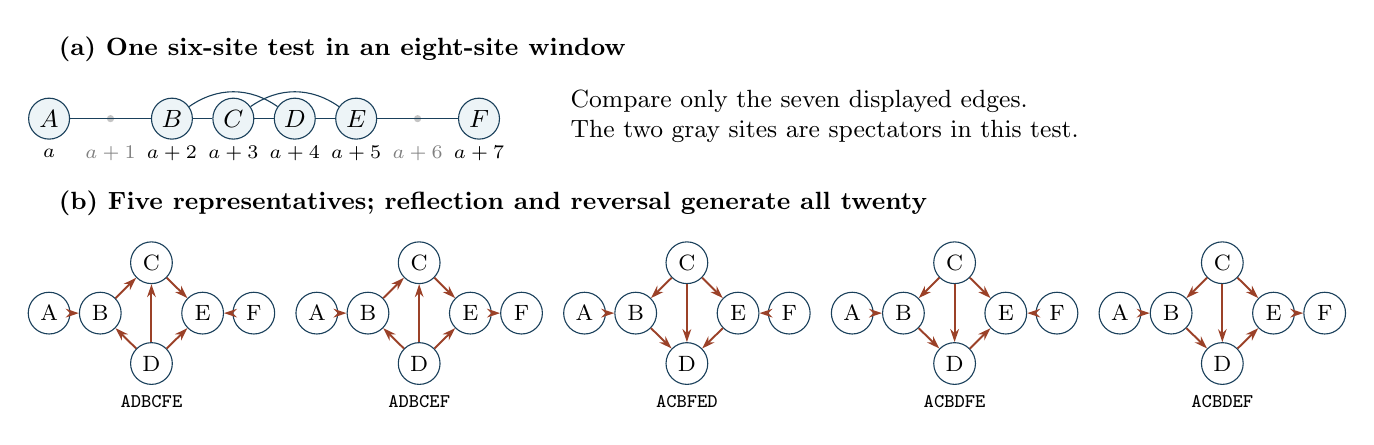
\begin{tikzpicture}[font=\small]
\node[anchor=west,font=\small\bfseries] at (0,2.1) {(a) One six-site test in an eight-site window};
\foreach \j/\lab in {0/A,2/B,3/C,4/D,5/E,7/F}{
 \node[circle,draw=deepblue,fill=softblue,inner sep=0pt,minimum size=5.2mm] (s\j) at (0.78*\j,1.22) {$\lab$};
 \node[font=\scriptsize] at (0.78*\j,0.78) {$\ifnum\j=0 a\else a+\j\fi$};}
\foreach \j in {1,6}{\fill[black!23] (0.78*\j,1.22) circle (1.3pt);\node[font=\scriptsize,text=black!50] at (0.78*\j,0.78) {$a+\j$};}
\foreach \a/\b in {0/2,2/3,3/4,4/5,5/7}{\draw[deepblue] (s\a)--(s\b);}
\draw[deepblue,bend left=35] (s2) to (s4);\draw[deepblue,bend left=35] (s3) to (s5);
\node[anchor=west,align=left,font=\small] at (6.5,1.25) {Compare only the seven displayed edges.\\The two gray sites are spectators in this test.};
\node[anchor=west,font=\small\bfseries] at (0,0.15) {(b) Five representatives; reflection and reversal generate all twenty};
\begin{scope}[shift={(0.0,-1.25)},x=1cm,y=1cm]
\foreach \v/\x/\y in {A/0/0,B/0.65/0,C/1.3/0.64,D/1.3/-0.64,E/1.95/0,F/2.6/0}{\node[circle,draw=deepblue,fill=white,inner sep=0pt,minimum size=5.3mm,font=\footnotesize] (\v) at (\x,\y) {\v};}
\draw[-{Stealth[length=1.65mm,width=1.1mm]},draw=rust,line width=0.7pt] (A)--(B);
\draw[-{Stealth[length=1.65mm,width=1.1mm]},draw=rust,line width=0.7pt] (B)--(C);
\draw[-{Stealth[length=1.65mm,width=1.1mm]},draw=rust,line width=0.7pt] (D)--(B);
\draw[-{Stealth[length=1.65mm,width=1.1mm]},draw=rust,line width=0.7pt] (D)--(C);
\draw[-{Stealth[length=1.65mm,width=1.1mm]},draw=rust,line width=0.7pt] (C)--(E);
\draw[-{Stealth[length=1.65mm,width=1.1mm]},draw=rust,line width=0.7pt] (D)--(E);
\draw[-{Stealth[length=1.65mm,width=1.1mm]},draw=rust,line width=0.7pt] (F)--(E);
\node[font=\scriptsize\ttfamily] at (1.3,-1.12) {ADBCFE};\end{scope}
\begin{scope}[shift={(3.4,-1.25)},x=1cm,y=1cm]
\foreach \v/\x/\y in {A/0/0,B/0.65/0,C/1.3/0.64,D/1.3/-0.64,E/1.95/0,F/2.6/0}{\node[circle,draw=deepblue,fill=white,inner sep=0pt,minimum size=5.3mm,font=\footnotesize] (\v) at (\x,\y) {\v};}
\draw[-{Stealth[length=1.65mm,width=1.1mm]},draw=rust,line width=0.7pt] (A)--(B);
\draw[-{Stealth[length=1.65mm,width=1.1mm]},draw=rust,line width=0.7pt] (B)--(C);
\draw[-{Stealth[length=1.65mm,width=1.1mm]},draw=rust,line width=0.7pt] (D)--(B);
\draw[-{Stealth[length=1.65mm,width=1.1mm]},draw=rust,line width=0.7pt] (D)--(C);
\draw[-{Stealth[length=1.65mm,width=1.1mm]},draw=rust,line width=0.7pt] (C)--(E);
\draw[-{Stealth[length=1.65mm,width=1.1mm]},draw=rust,line width=0.7pt] (D)--(E);
\draw[-{Stealth[length=1.65mm,width=1.1mm]},draw=rust,line width=0.7pt] (E)--(F);
\node[font=\scriptsize\ttfamily] at (1.3,-1.12) {ADBCEF};\end{scope}
\begin{scope}[shift={(6.8,-1.25)},x=1cm,y=1cm]
\foreach \v/\x/\y in {A/0/0,B/0.65/0,C/1.3/0.64,D/1.3/-0.64,E/1.95/0,F/2.6/0}{\node[circle,draw=deepblue,fill=white,inner sep=0pt,minimum size=5.3mm,font=\footnotesize] (\v) at (\x,\y) {\v};}
\draw[-{Stealth[length=1.65mm,width=1.1mm]},draw=rust,line width=0.7pt] (A)--(B);
\draw[-{Stealth[length=1.65mm,width=1.1mm]},draw=rust,line width=0.7pt] (C)--(B);
\draw[-{Stealth[length=1.65mm,width=1.1mm]},draw=rust,line width=0.7pt] (B)--(D);
\draw[-{Stealth[length=1.65mm,width=1.1mm]},draw=rust,line width=0.7pt] (C)--(D);
\draw[-{Stealth[length=1.65mm,width=1.1mm]},draw=rust,line width=0.7pt] (C)--(E);
\draw[-{Stealth[length=1.65mm,width=1.1mm]},draw=rust,line width=0.7pt] (E)--(D);
\draw[-{Stealth[length=1.65mm,width=1.1mm]},draw=rust,line width=0.7pt] (F)--(E);
\node[font=\scriptsize\ttfamily] at (1.3,-1.12) {ACBFED};\end{scope}
\begin{scope}[shift={(10.2,-1.25)},x=1cm,y=1cm]
\foreach \v/\x/\y in {A/0/0,B/0.65/0,C/1.3/0.64,D/1.3/-0.64,E/1.95/0,F/2.6/0}{\node[circle,draw=deepblue,fill=white,inner sep=0pt,minimum size=5.3mm,font=\footnotesize] (\v) at (\x,\y) {\v};}
\draw[-{Stealth[length=1.65mm,width=1.1mm]},draw=rust,line width=0.7pt] (A)--(B);
\draw[-{Stealth[length=1.65mm,width=1.1mm]},draw=rust,line width=0.7pt] (C)--(B);
\draw[-{Stealth[length=1.65mm,width=1.1mm]},draw=rust,line width=0.7pt] (B)--(D);
\draw[-{Stealth[length=1.65mm,width=1.1mm]},draw=rust,line width=0.7pt] (C)--(D);
\draw[-{Stealth[length=1.65mm,width=1.1mm]},draw=rust,line width=0.7pt] (C)--(E);
\draw[-{Stealth[length=1.65mm,width=1.1mm]},draw=rust,line width=0.7pt] (D)--(E);
\draw[-{Stealth[length=1.65mm,width=1.1mm]},draw=rust,line width=0.7pt] (F)--(E);
\node[font=\scriptsize\ttfamily] at (1.3,-1.12) {ACBDFE};\end{scope}
\begin{scope}[shift={(13.6,-1.25)},x=1cm,y=1cm]
\foreach \v/\x/\y in {A/0/0,B/0.65/0,C/1.3/0.64,D/1.3/-0.64,E/1.95/0,F/2.6/0}{\node[circle,draw=deepblue,fill=white,inner sep=0pt,minimum size=5.3mm,font=\footnotesize] (\v) at (\x,\y) {\v};}
\draw[-{Stealth[length=1.65mm,width=1.1mm]},draw=rust,line width=0.7pt] (A)--(B);
\draw[-{Stealth[length=1.65mm,width=1.1mm]},draw=rust,line width=0.7pt] (C)--(B);
\draw[-{Stealth[length=1.65mm,width=1.1mm]},draw=rust,line width=0.7pt] (B)--(D);
\draw[-{Stealth[length=1.65mm,width=1.1mm]},draw=rust,line width=0.7pt] (C)--(D);
\draw[-{Stealth[length=1.65mm,width=1.1mm]},draw=rust,line width=0.7pt] (C)--(E);
\draw[-{Stealth[length=1.65mm,width=1.1mm]},draw=rust,line width=0.7pt] (D)--(E);
\draw[-{Stealth[length=1.65mm,width=1.1mm]},draw=rust,line width=0.7pt] (E)--(F);
\node[font=\scriptsize\ttfamily] at (1.3,-1.12) {ACBDEF};\end{scope}
\end{tikzpicture}
\caption{\textbf{The forbidden heaps.} A representative word specifies only relative orders on the seven edges of $H$; adjacent commuting letters may be exchanged freely. Each panel in (b) represents four distinct orientations under temporal reversal and spatial reflection. Applying this test at every position gives the exact canonical classification.}
\label{L:badfig}
\end{figure*}

\paragraph{Why the criterion works.}
Necessity is genuinely local. Turn off all gates outside a forbidden copy by setting their angles to zero. In its six-generator algebra, the full-support coefficient of $[Q_1,Q_3]$, where $\cA(z)=\sum_r z^rQ_r$, is nonzero. For the five representatives it is, after division by $\prod_{X=A}^Fy_X$, respectively
\begin{equation}\label{L:obstruction}
 -2x_E,\quad-2x_F,\quad2x_D,\quad2x_E,\quad2x_F.
\end{equation}

Sufficiency has a geometric reduction. The nullity is the number of connected components of $F_M[S]$ plus the nullity of an auxiliary graph whose vertices are the selected consecutive triangles. Two such triangles are linked according to the temporal order of their middle events. Avoidance forces this auxiliary graph to be a union of paths. A path contributes one to the nullity precisely when it contains an odd number of vertices. Consequently
\begin{equation}\label{L:pathgrade}
 \nu_D(S)=c(F_M[S])+\#\{\text{odd interlace paths}\}.
\end{equation}
Only a fixed frontier must be remembered as the chain is scanned; a 32-state transducer evaluates the grade.

Every angle coefficient of the commutator and of the noncentral inversion product then becomes a signed weighted sum recognized by a finite automaton. Exact quotients have $9{,}756$ and $7{,}195$ states. Their vanishing is certified by invariant subspaces of dimensions $590$ and $427$ over $\mathbb Q(z,w)$ and $\mathbb Q(z)$, respectively. The full verification checks all $17{,}700+12{,}810$ transition images. This is an all-length proof, not an extrapolation from short chains. The supplementary material gives the reductions, the finite-state definitions, and executable pseudocode.

\paragraph{From the transfer polynomial to the spectrum.}
Fix a central sector $\chi$. Central inversion becomes
\begin{equation}\label{L:sectorinv}
 \cA_{D,\chi}(z)\cA_{D,\chi}(-z)=p_{D,\chi}(z)\one.
\end{equation}
For generic angles, $p_{D,\chi}$ has $s_M$ distinct nonzero root pairs $\{r_{\chi,k},-r_{\chi,k}\}$. Simultaneous diagonalization and \eqref{L:sectorinv} give
\begin{equation}\label{L:spectrum}
 \boxed{v_{\chi,\boldsymbol\sigma}
 =a_0\prod_{k=1}^{s_M}\left(1+\frac{\sigma_k}{r_{\chi,k}}\right),
 \qquad\boldsymbol\sigma\in\mathcal C_\chi.}
\end{equation}
The admissible signs form an affine binary code with equal multiplicities. In a fixed irreducible sector they are unrestricted unless $M\equiv1\pmod3$; in that case one product-of-signs constraint remains. Its value is obtained from the highest transfer coefficient, as explained in Sec.~\ref{supp:roots}.

For real angles on the generic locus, choose $r_{\chi,k}=iu_{\chi,k}$ with $u_{\chi,k}>0$. Changing the $k$th sign from $-1$ to $+1$ multiplies the eigenvalue by
\begin{equation}\label{L:phase}
 q_{\chi,k}=\frac{iu_{\chi,k}+1}{iu_{\chi,k}-1}
 =e^{-i\omega_{\chi,k}},\quad
 \omega_{\chi,k}=2\arctan\frac1{u_{\chi,k}}.
\end{equation}
A fixed-sector parity constraint may require signs to change in pairs. The displayed quantities are the elementary factors, not a claim that every individual flip is allowed in each sector.

\paragraph{Computing the polynomial, not a large matrix.}
The identity coefficient of the inversion product is the positive sum
\begin{equation}\label{L:scalar}
 p_0(z)=\sum_{S\text{ feasible}}z^{2\nu_D(S)}
 \prod_{j\in S}y_j^2\!
 \prod_{\substack{j\notin S\\e_D(j,S)=0}}x_j^2.
\end{equation}
When inversion is scalar in the full algebra, $p_0=p_{D,\chi}$ for every sector. \emph{Centrality alone is not enough to make this replacement.} In general one also computes the coefficients supported on $\ker_{\FF}A_M$, where $A_M$ is the frustration adjacency matrix, and evaluates them in $\chi$. This kernel has dimension at most two. A paired version of the same frontier scan computes all sector polynomials in $O(Ms_M)$ arithmetic operations, with a size-independent state bound (Sec.~\ref{supp:sectoralgorithm}). Thus the general root prescription is constructive even when the center is nontrivial.

The familiar half-words I, II, and III are
\begin{equation}\label{L:families}
 \begin{aligned}
 \mathrm I &: (1,2,\ldots,M),\\
 \mathrm {II} &: (2,4,\ldots,M;1,3,\ldots,M-1),\\
 \mathrm {III} &: (3,6,\ldots,M;2,5,\ldots,M-1;1,4,\ldots,M-2),
 \end{aligned}
\end{equation}
with the usual even-$M$ and $3\mid M$ conventions in II and III. They pass the local test. These are the regular families solved in Ref.~\cite{SzaszSchagrinEtAl2026}; the present construction also covers heaps without a repeating architecture.

As a nonperiodic example, take $M=9$, $\pi=(9,4,2,5,7,1,3,8,6)$, and $\phi_j=0.17+0.029(j-1)+0.004\sin j$. Direct evaluation verifies scalar inversion here. The normalized mode polynomial $P(x)=p_0(i\sqrt{x})/p_0(0)$ is
\begin{equation}\label{L:example}
 \begin{aligned}
 P(x)={}&1-1.02263185775715x\\
       &+0.209346393878477x^2\\
       &-0.00725922352756874x^3.
 \end{aligned}
\end{equation}
The roots are approximately $1.31645$, $4.55642$, and $22.96581$, with occupation-flip phases $1.433758$, $0.876225$, and $0.411435$. Using unrounded coefficients, the eight eigenvalues from \eqref{L:spectrum}, each with multiplicity $64$, agree with an independent $512\times512$ spin-circuit calculation to $1.2\times10^{-14}$.

\paragraph{Scope.}
The result resolves the ordering problem for the canonical nullity-graded transfer construction: acceptance is both necessary and sufficient, and supplies a polynomial-root solution. It does not turn failure of that particular construction into a no-go theorem for every other definition of free-fermion solvability. Repeated roots, vanishing cosines, and other nongeneric points are obtained by limits of the unnormalized polynomial identities; normalized root formulas should not be used there without taking those limits.

\paragraph{Reproducibility.}
The accompanying single-file code archive contains the complete proof sources and certificates, a sector-aware spectral solver, and independent checks. Both formal automata were regenerated byte for byte, all characteristic-zero certificate identities were rerun, and the independent finite audits were repeated. No finite-field specialization is used as the final proof.

\begin{thebibliography}{9}\small
\bibitem{Fendley2019} P. Fendley, Free fermions in disguise, J. Phys. A: Math. Theor. \textbf{52}, 335002 (2019), \href{https://arxiv.org/abs/1901.08078}{arXiv:1901.08078}.
\bibitem{ElmanChapmanFlammia2021} S. J. Elman, A. Chapman, and S. T. Flammia, Free fermions behind the disguise, Commun. Math. Phys. \textbf{388}, 969--1003 (2021), \href{https://arxiv.org/abs/2012.07857}{arXiv:2012.07857}.
\bibitem{PozsgayFukai2025} K. Fukai and B. Pozsgay, Quantum circuits with free fermions in disguise, J. Phys. A: Math. Theor. \textbf{58}, 175202 (2025), \href{https://arxiv.org/abs/2402.02984}{arXiv:2402.02984}.
\bibitem{SzaszSchagrinEtAl2026} D. Sz\'asz-Schagrin, D. Cristani, L. Piroli, and E. Vernier, Construction and simulability of quantum circuits with free fermions in disguise, Quantum Sci. Technol. \textbf{11}, 015044 (2026), \href{https://arxiv.org/abs/2509.22585}{arXiv:2509.22585}.
\bibitem{CartierFoata1969} P. Cartier and D. Foata, \emph{Probl\`emes combinatoires de commutation et r\'earrangements}, Lecture Notes in Mathematics \textbf{85} (Springer, 1969).
\bibitem{BerstelReutenauer2011} J. Berstel and C. Reutenauer, \emph{Noncommutative Rational Series with Applications} (Cambridge University Press, 2011).
\end{thebibliography}

\clearpage\onecolumn
\setcounter{page}{1}\renewcommand{\thepage}{S\arabic{page}}
\setcounter{section}{0}\renewcommand{\thesection}{S\arabic{section}}
\setcounter{equation}{0}\renewcommand{\theequation}{S\arabic{equation}}
\setcounter{theorem}{0}\renewcommand{\thetheorem}{S\arabic{theorem}}
\setcounter{figure}{0}\renewcommand{\thefigure}{S\arabic{figure}}
\setcounter{table}{0}\renewcommand{\thetable}{S\arabic{table}}
\setcounter{algorithm}{0}\renewcommand{\thealgorithm}{S\arabic{algorithm}}
\fancyhead[L]{\footnotesize SUPPLEMENTARY MATERIAL}\fancyhead[R]{\footnotesize Forbidden heaps and FFD spectra}
\renewcommand{\headrulewidth}{0.25pt}
\begin{center}
{\Large\bfseries Supplementary material}\\[0.4em]
{\large Forbidden heaps and the spectral solution of free-fermion-in-disguise circuits}
\end{center}
\noindent This supplement contains the complete algebraic reductions, the finite exact certificate argument, and the constructive sector-by-sector spectral solution. The long-chain cancellations use the finite exact certificates included in the archive. The final sections document the independently rerun checks and the accompanying code archive.
\vspace{0.6em}
\section{Open FFD circuits and heaps}\label{sec:setup}

\subsection{The algebra}

Fix \(M\ge1\).  The open FFD \(*\)-algebra \(\Aalg_M\) is generated by Hermitian involutions \(h_1,\ldots,h_M\) satisfying
\begin{equation}\label{eq:ffd-algebra}
 h_j^2=\one,
 \qquad
 \{h_j,h_k\}=0 \quad (1\le |j-k|\le2),
 \qquad
 [h_j,h_k]=0 \quad (|j-k|>2).
\end{equation}
The frustration graph is
\[
 F_M=P_M^2,
 \qquad
 \{j,k\}\in E(F_M)\Longleftrightarrow 1\le|j-k|\le2.
\]
The open chain and its distance-one and distance-two frustration edges are illustrated in \cref{fig:ffd-graph}.

\begin{figure}[H]
\centering
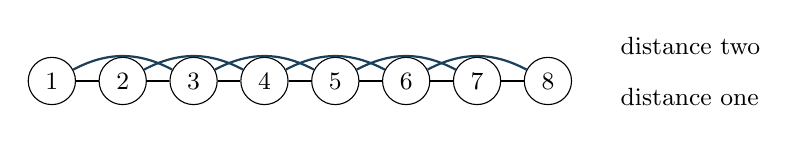
\begin{tikzpicture}[
 v/.style={circle,draw,minimum size=6mm,inner sep=0pt,font=\small},
 e1/.style={thick},e2/.style={thick,draw=deepblue,bend left=28}
]
\foreach \x in {1,...,8}{\node[v] (v\x) at (0.9*\x,0) {\x};}
\foreach \x [evaluate=\x as \y using int(\x+1)] in {1,...,7}{\draw[e1] (v\x)--(v\y);}
\foreach \x [evaluate=\x as \y using int(\x+2)] in {1,...,6}{\draw[e2] (v\x) to (v\y);}
\node[align=left,anchor=west,font=\small] at (8.0,0.45) {distance two};
\node[align=left,anchor=west,font=\small] at (8.0,-0.2) {distance one};
\end{tikzpicture}
\caption{The frustration graph \(F_M=P_M^2\).  Generators anticommute along both kinds of edge and commute otherwise.}
\label{fig:ffd-graph}
\end{figure}

Choose a spatial normal order \(h^x=h_1^{x_1}\cdots h_M^{x_M}\) for \(x\in\FF^M\).  If \(A_M\) is the adjacency matrix of \(F_M\) over \(\FF\), then
\begin{equation}\label{eq:comm-form}
 h^x h^y=(-1)^{x^{\mathsf T}A_My}h^yh^x.
\end{equation}
Hence \(h^x\) is central exactly when \(A_Mx=0\).  We write \(\Zalg_M=Z(\Aalg_M)\).

\subsection{Palindromic permutation circuits}

For real angles \(\phi_j\), define
\begin{equation}\label{eq:gate}
 u_j=\exp\!\left(\frac{i\phi_j}{2}h_j\right)
 =\cos\!\left(\frac{\phi_j}{2}\right)\one
 +i\sin\!\left(\frac{\phi_j}{2}\right)h_j.
\end{equation}
Let \(T\) be the complex-linear anti-involution determined by \(h_j^T=h_j\) and \((XY)^T=Y^TX^T\).  For a permutation \(\pi=(\pi_1,\ldots,\pi_M)\), set
\begin{equation}\label{eq:palindrome}
 G_\pi=u_{\pi_1}\cdots u_{\pi_M},
 \qquad
 V_\pi=G_\pi G_\pi^T.
\end{equation}
Thus the second half retraces the first without complex conjugating the scalar \(i\).  The circuit is a one-pass palindrome: every generator occurs once in the half-word.

\begin{figure}[H]
\centering
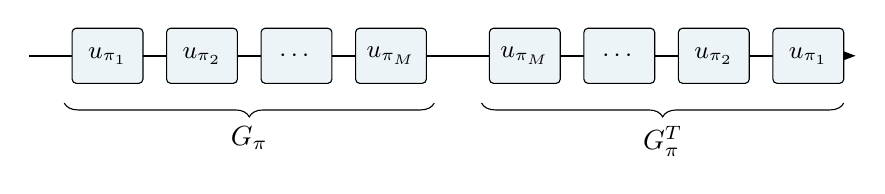
\begin{tikzpicture}[
 gate/.style={draw,rounded corners=1.5pt,minimum width=9mm,minimum height=7mm,fill=softblue,font=\small},
 arr/.style={-{Stealth[length=2mm]},thick}
]
\draw[arr] (0,0)--(10.5,0);
\foreach \x/\lab in {1/u_{\pi_1},2.2/u_{\pi_2},3.4/\cdots,4.6/u_{\pi_M},6.3/u_{\pi_M},7.5/\cdots,8.7/u_{\pi_2},9.9/u_{\pi_1}}{
  \node[gate] at (\x,0) {$\lab$};
}
\draw[decorate,decoration={brace,mirror,amplitude=5pt}] (0.45,-0.6)--(5.15,-0.6) node[midway,below=5pt] {$G_\pi$};
\draw[decorate,decoration={brace,mirror,amplitude=5pt}] (5.75,-0.6)--(10.35,-0.6) node[midway,below=5pt] {$G_\pi^T$};
\end{tikzpicture}
\caption{The palindromic circuit \(V_\pi=G_\pi G_\pi^T\).  Only the relative order of noncommuting gates matters.}
\label{fig:palindrome}
\end{figure}

\subsection{Heaps: order modulo commuting swaps}

Orient every edge \(j-k\) of \(F_M\) from the label that occurs earlier in \(\pi\) to the label that occurs later.  The result is an acyclic orientation \(D_\pi\).  Two permutations determine the same orientation exactly when they differ by adjacent exchanges of commuting labels.  Since those gates commute, the circuit depends only on the orientation.  We call it the \emph{heap} \(D\), following the trace-monoid viewpoint \citep{CartierFoata1969}.

We write \(v\to w\) when the edge \(vw\) is directed from \(v\) to \(w\).  The directed adjacency matrix is
\begin{equation}\label{eq:directed-adj}
 (E_D)_{vw}=\mathbf1_{\{v\to w\}}.
\end{equation}
Then \(E_D+E_D^{\mathsf T}=A_M\).

A convenient insertion encoding will be used by the automata.  After the first edge is oriented, a new site \(j\) belongs to the triangle \(j-2,j-1,j\).  Transitivity allows exactly three temporal positions: before both old sites, between them, or after both.  We denote this ternary choice by \(q_j\in\{0,1,2\}\).  Consequently the number of acyclic orientations is \(2\cdot3^{M-2}\) for \(M\ge2\).

\section{Exact expansion of the palindrome}\label{sec:expansion}

Put
\begin{equation}\label{eq:xy}
 x_j=\cos\phi_j,
 \qquad
 y_j=\sin\phi_j.
\end{equation}
The doubled gate is \(u_j^2=x_j+i y_jh_j\).  The exact expansion is most transparent if the palindrome is peeled from its outside.

For \(S\subseteq[M]\), define the selected outdegree parity
\begin{equation}\label{eq:out-parity}
 e_D(v,S)=\#\{w\in S:v\to w\}\pmod2.
\end{equation}

\begin{definition}[Feasible support]\label{def:feasible}
A support \(S\subseteq[M]\) is \(D\)-feasible if
\begin{equation}\label{eq:feasible}
 e_D(v,S)=0 \qquad (v\in S).
\end{equation}
We denote the family by \(\Ffam(D)\).
\end{definition}

For \(S\in\Ffam(D)\), let \(H_D(S)\) be the product of the selected generators in any linear extension of \(D|_S\).  This is well defined because incomparable vertices are nonadjacent in \(F_M\) and hence commute.

\begin{proposition}[Exact feasible-support expansion]\label{prop:exact-expansion}
The palindrome associated with a heap \(D\) is
\begin{equation}\label{eq:exact-expansion}
 V_D=\sum_{S\in\Ffam(D)}a_D(S)H_D(S),
\end{equation}
where
\begin{equation}\label{eq:coefficient-a}
 a_D(S)=i^{|S|}
 \prod_{v\in S}y_v
 \prod_{\substack{v\notin S\\ e_D(v,S)=0}}x_v.
\end{equation}
\end{proposition}

\begin{proof}
Let \(P\) be a graph-Clifford monomial in the generators that lie inside the current pair of gates.  Direct multiplication gives
\begin{equation}\label{eq:peel}
 u_vPu_v=
 \begin{cases}
 (x_v+i y_vh_v)P,&[h_v,P]=0,\\
 P,&\{h_v,P\}=0.
 \end{cases}
\end{equation}
The commutation parity of \(h_v\) with the later selected monomial is exactly \(e_D(v,S)\).  If it is odd, the two scalar terms and the two \(h_v\)-terms cancel pairwise, leaving \(P\); hence \(v\) must be absent.  If it is even, one may omit \(v\) with factor \(x_v\), or select it with factor \(iy_v\).  A selected vertex is therefore allowed exactly under \eqref{eq:feasible}.  Multiplying the local factors yields \eqref{eq:coefficient-a}.
\end{proof}

\begin{remark}[Why feasibility is temporal]
The condition is not merely even degree in the induced frustration graph.  Only later selected neighbors enter.  It therefore depends on the heap orientation.  This asymmetry is what permits nonstable feasible supports and is the source of the nontrivial grading below.
\end{remark}

\section{The temporal-footprint grading}\label{sec:grading}

The correct spectral degree is not \(|S|\).  Folded FFD circuits contain composite monomials, including trilinear terms, that carry degree one.  The nullity below supplies a grading compatible with the temporal overlap of the selected gates.

\subsection{Temporal adjacency and predecessor footprints}

Let \(S\in\Ffam(D)\), and list its elements in temporal order,
\[
 S=\{s_1\prec s_2\prec\cdots\prec s_n\}.
\]
Define the strictly upper-triangular matrix \(N=N_{D,S}\in M_n(\FF)\) by
\begin{equation}\label{eq:N}
 N_{ab}=\mathbf1_{\{a<b,\;1\le|s_a-s_b|\le2\}}.
\end{equation}
Thus row \(a\) records the later selected generators that anticommute with \(h_{s_a}\), and feasibility is
\begin{equation}\label{eq:N-feasible}
 N\one=0.
\end{equation}

For the later event \(s_a\), define its closed predecessor footprint
\begin{equation}\label{eq:footprint}
 p_a=\ee_a+\sum_{c<a}N_{ca}\ee_c.
\end{equation}
The footprint marks the event itself and every earlier selected event whose commutation parity is flipped by selecting \(s_a\).  If the footprints are placed as columns, then
\begin{equation}\label{eq:B}
 B=(p_1\ \cdots\ p_n)=I+N.
\end{equation}
Their binary Gram matrix is
\begin{equation}\label{eq:Gram}
 G=B^{\mathsf T}B=I+N+N^{\mathsf T}+N^{\mathsf T}N.
\end{equation}
The diagonal of \(G\) is unavoidable self-overlap.  Since \(B\) is unitriangular, \(G\) is always nonsingular and its full nullity is trivial.  The mutual overlaps are captured by deleting the diagonal.

\begin{definition}[Canonical grading matrix]\label{def:K}
Set
\begin{equation}\label{eq:K}
 K_D(S)=\offdiag\!\left[(I+N_{D,S})^{\mathsf T}(I+N_{D,S})\right]
 =N+N^{\mathsf T}+\offdiag(N^{\mathsf T}N),
\end{equation}
and define
\begin{equation}\label{eq:nu}
 \nu_D(S)=\nullity_{\FF}K_D(S).
\end{equation}
\end{definition}

For \(a\ne b\), the entry has the explicit form
\begin{equation}\label{eq:K-entry}
 (K_D(S))_{ab}
 =\mathbf1_{\{s_a\sim s_b\}}
 +\#\{c:s_c\prec s_a,s_b,\ s_c\sim s_a,s_b\}\pmod2.
\end{equation}
The first term is direct anticommutation.  The second counts common temporal predecessors: two later selected events overlap when they flip the same earlier parity register.

\begin{figure}[t]
\centering
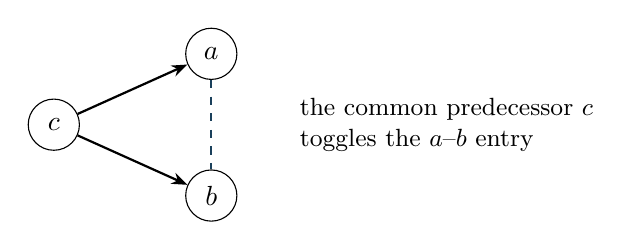
\begin{tikzpicture}[
 v/.style={circle,draw,minimum size=6.5mm,inner sep=0pt},
 arr/.style={-{Stealth[length=2mm]},thick},
 toggle/.style={thick,dashed,draw=deepblue}
]
\node[v] (c) at (0,0) {$c$};
\node[v] (a) at (2,0.9) {$a$};
\node[v] (b) at (2,-0.9) {$b$};
\draw[arr] (c)--(a);
\draw[arr] (c)--(b);
\draw[toggle] (a)--(b);
\node[align=left,anchor=west,font=\small] at (3.0,0) {the common predecessor \(c\)\\toggles the \(a\)--\(b\) entry};
\end{tikzpicture}
\caption{A temporal fork.  The two arrows contribute \(N_{ca}N_{cb}=1\), so the common-predecessor term toggles the mutual relation of \(a\) and \(b\).}
\label{fig:temporal-fork}
\end{figure}

\begin{example}[One temporal fork]
For
\[
 N=\begin{pmatrix}0&1&1\\0&0&0\\0&0&0\end{pmatrix},
\]
the direct frustration graph is a two-leaf star.  The common predecessor adds the leaf-to-leaf edge, and
\[
 K=\begin{pmatrix}0&1&1\\1&0&1\\1&1&0\end{pmatrix}
\]
has binary nullity one.  Thus this feasible trilinear monomial has spectral degree one.
\end{example}

\subsection{Elementary properties}

\begin{lemma}[Basic grading properties]\label{lem:grade-basic}
For every feasible support \(S\):
\begin{enumerate}[label=\textup{(\alph*)}]
\item \(\nu_D(S)\) is independent of the chosen linear extension;
\item \(K_D(S)\one=0\);
\item \(\nu_D(S)\equiv|S|\pmod2\);
\item \(H_D(S)\) is Hermitian.
\end{enumerate}
\end{lemma}

\begin{proof}
Adjacent exchanges between linear extensions involve incomparable, hence nonadjacent, vertices.  They only permute matching rows and columns of \(K_D(S)\), proving (a).

For (b), feasibility gives \(N\one=0\).  Over \(\FF\),
\[
 \diag(N^{\mathsf T}N)=N^{\mathsf T}\one,
 \qquad
 \offdiag(N^{\mathsf T}N)\one=N^{\mathsf T}\one.
\]
Therefore
\[
 K_D(S)\one=N\one+N^{\mathsf T}\one+N^{\mathsf T}\one=0.
\]
The matrix \(K_D(S)\) is symmetric with zero diagonal, hence alternating over \(\FF\).  Its rank is even, which proves (c).

Reversing \(H_D(S)\) introduces one minus sign for every edge of \(F_M[S]\).  The number of such edges is the sum of the selected outdegrees in \(D[S]\), which is even by feasibility.  Hence the monomial is Hermitian, proving (d).
\end{proof}

The identity \(K_D(S)\one=0\) is also a useful retrospective explanation for the correction \(N^{\mathsf T}N\).  The direct frustration matrix \(N+N^{\mathsf T}\) need not be singular on a feasible support.  The common-predecessor term cancels its residual column-parity vector exactly.

\subsection{The canonical Baxter family}

\begin{definition}[Canonical family]\label{def:canonical-family}
Define
\begin{equation}\label{eq:canonical-A}
 \boxed{\displaystyle
 \cA_D(z)=\sum_{S\in\Ffam(D)}a_D(S)z^{\nu_D(S)}H_D(S)
 =\sum_{r\ge0}z^rQ_{D,r}.}
\end{equation}
\end{definition}
By construction,
\begin{equation}\label{eq:endpoints}
 \cA_D(1)=V_D,
 \qquad
 \cA_D(0)=a_0\one,
 \qquad
 a_0=\prod_{j=1}^M x_j.
\end{equation}
The last identity uses \(K_D(S)\one=0\): every nonempty feasible support has positive nullity.

\begin{corollary}[Adjoint parity]\label{cor:adjoint}
For every \(r\),
\begin{equation}\label{eq:charge-adjoint}
 Q_{D,r}^{\dagger}=(-1)^rQ_{D,r}.
\end{equation}
Consequently \(\cA_D(z)^\dagger=\cA_D(-z)\) for real \(z\).
\end{corollary}

\begin{proof}
The only nonreal factor in \(a_D(S)\) is \(i^{|S|}\).  By \cref{lem:grade-basic}, \(|S|\equiv\nu_D(S)\pmod2\), while \(H_D(S)\) is Hermitian.  Group terms of fixed nullity.
\end{proof}

\section{Forbidden heaps and the Baxter property}\label{sec:forbidden}

\subsection{The six-vertex obstruction}

Let \(H\) have vertices \(A,B,C,D,E,F\) and edges
\begin{equation}\label{eq:H-edges}
 E(H)=\{AB,BC,BD,CD,CE,DE,EF\}.
\end{equation}
It consists of two triangles \(BCD\) and \(CDE\) sharing the edge \(CD\), with pendant edges \(AB\) and \(EF\).

\begin{figure}[t]
\centering
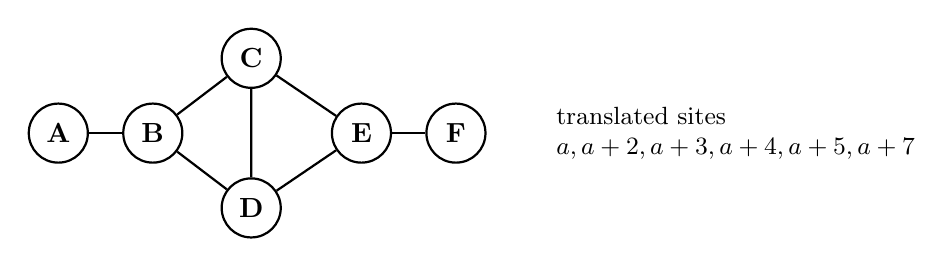
\begin{tikzpicture}[
 vertex/.style={circle,draw,thick,minimum size=7.5mm,inner sep=0pt,font=\bfseries},
 arr/.style={-{Stealth[length=2mm]},thick},
 plain/.style={thick}
]
\node[vertex] (A) at (-3.2,0) {A};
\node[vertex] (B) at (-2.0,0) {B};
\node[vertex] (C) at (-0.75,0.95) {C};
\node[vertex] (D) at (-0.75,-0.95) {D};
\node[vertex] (E) at (0.65,0) {E};
\node[vertex] (F) at (1.85,0) {F};
\draw[plain] (A)--(B);
\draw[plain] (B)--(C)--(D)--(B);
\draw[plain] (C)--(E)--(D);
\draw[plain] (E)--(F);
\node[font=\small,align=left,anchor=west] at (3.0,0) {translated sites\\\(a,a+2,a+3,a+4,a+5,a+7\)};
\end{tikzpicture}
\caption{The obstruction graph \(H\).  Twenty of its seventy-two acyclic orientations are forbidden.}
\label{fig:H-obstruction}
\end{figure}

For a word containing the six letters once, orient every edge from the earlier letter to the later one.  Let \(\tau\) reverse the word, and let \(\rho\) be the spatial reflection
\[
 A\leftrightarrow F,
 \qquad B\leftrightarrow E,
 \qquad C\leftrightarrow D.
\]
Start from the five temporal orders
\begin{equation}\label{eq:H-reps}
 ADB CFE,
 \qquad ADB CEF,
 \qquad ACB FED,
 \qquad ACB DFE,
 \qquad ACB DEF,
\end{equation}
where spaces are inserted only for readability.  Applying \(\tau^\epsilon\rho^\delta\), \(\epsilon,\delta\in\{0,1\}\), gives twenty distinct orientations.  Their set is denoted \(\mathfrak B\).  A complete seven-bit signature list is given in \cref{app:forbidden-list}.

For \(1\le a\le M-7\), the sites
\begin{equation}\label{eq:H-translate}
 A=a,
 \quad B=a+2,
 \quad C=a+3,
 \quad D=a+4,
 \quad E=a+5,
 \quad F=a+7
\end{equation}
induce a copy \(H_a\subset P_M^2\).

\begin{definition}[\(H\)-avoidance]
A heap \(D\) is \(H\)-avoiding if \(D|_{H_a}\notin\mathfrak B\) for every allowed translation \(a\).
\end{definition}

\subsection{Canonical Baxter property}

Let
\begin{equation}\label{eq:sM}
 s_M=\alpha(P_M^2)=\left\lceil\frac M3\right\rceil.
\end{equation}
All angle identities are understood in the quotient ring
\begin{equation}\label{eq:angle-ring}
 \mathscr R_M=
 \mathbb C[x_1,y_1,\ldots,x_M,y_M]
 /(x_j^2+y_j^2-1:1\le j\le M).
\end{equation}

\begin{definition}[Canonical Baxter property]\label{def:baxter}
A heap \(D\) has the canonical Baxter property if
\begin{align}
 \deg_z\cA_D(z)&\le s_M,\label{eq:bax-degree}\\
 [\cA_D(z),\cA_D(w)]&=0,\label{eq:bax-comm}\\
 \cA_D(z)\cA_D(-z)&\in\Zalg_M[z^2].\label{eq:bax-inv}
\end{align}
\end{definition}

\Cref{thm:main} says that this property is equivalent to avoiding the twenty local orientations.

\section{Physical consequence: a product spectrum}\label{sec:spectrum}

The algebraic theorem immediately implies the usual free-fermion spectral form.  We include the derivation because it explains why the three Baxter conditions are the right target.

An \emph{affine sign code} \(\mathcal C\subseteq\{\pm1\}^s\) is a coset of a subgroup under componentwise multiplication; equivalently, it is defined by parity equations
\[
 \prod_{k=1}^s\sigma_k^{c_{\ell k}}=\zeta_\ell,
 \qquad c_{\ell k}\in\FF,
 \quad \zeta_\ell\in\{\pm1\}.
\]

\begin{theorem}[Baxter identities and the FFD spectrum]\label{thm:baxter-spectrum}
Suppose \(D\) has the canonical Baxter property.  On a Zariski-open set of angle parameters, the following holds in every irreducible central sector \(\chi\).  The charges have a common, \(z\)-independent eigenspace decomposition, and their joint eigenvalue polynomials are
\begin{equation}\label{eq:product-spectrum}
 \Lambda_{\chi,\bm\sigma}(z)
 =a_0\prod_{k=1}^{s_M}(1+\sigma_k\lambda_{\chi,k}z),
 \qquad \bm\sigma\in\mathcal C_\chi,
\end{equation}
where the nonzero \(\lambda_{\chi,k}\) are distinct up to sign, \(\mathcal C_\chi\) is an affine sign code, and every allowed sign vector occurs with the same multiplicity.  Conversely, a common eigenbasis with the product form \eqref{eq:product-spectrum} implies the canonical Baxter property.
\end{theorem}

\begin{proof}
By \cref{cor:adjoint}, the operators \(i^{-r}Q_{D,r}\) are Hermitian.  Commutation therefore gives a common eigenbasis in each central sector.  Let \(\Lambda_a(z)\) be one joint eigenvalue polynomial.  The degree and constant term obey
\[
 \deg\Lambda_a\le s_M,
 \qquad \Lambda_a(0)=a_0.
\]
Central inversion becomes a scalar identity
\begin{equation}\label{eq:scalar-inversion}
 \Lambda_a(z)\Lambda_a(-z)=P_\chi(z^2),
\end{equation}
with the same polynomial \(P_\chi\) for every joint eigenspace in the sector.

To see the generic root structure, specialize all angles outside the maximal stable set
\[
 I=\{1,4,7,\ldots\}\cap[M],
 \qquad |I|=s_M,
\]
to \(y_j=0,x_j=1\).  Every surviving support lies in \(I\), so \(N=K=0\) and \(\nu_D(S)=|S|\).  Hence, independently of the heap,
\begin{equation}\label{eq:decoupled-A}
 \cA_D(z)=\prod_{j\in I}(x_j+i z y_jh_j),
\end{equation}
and
\[
 P_\chi(z^2)=\prod_{j\in I}(x_j^2+y_j^2z^2).
\]
At generic values this polynomial has \(s_M\) distinct nonzero root pairs.  Therefore, away from a proper algebraic subset,
\begin{equation}\label{eq:P-factor}
 P_\chi(z^2)=a_0^2\prod_{k=1}^{s_M}(1-\lambda_{\chi,k}^2z^2).
\end{equation}
A polynomial \(\Lambda_a\) satisfying \eqref{eq:scalar-inversion} contains exactly one zero from every pair \(\{\lambda_{\chi,k}^{-1},-\lambda_{\chi,k}^{-1}\}\).  It cannot contain both, because that would make a double zero in the product, and it cannot contain neither.  This proves \eqref{eq:product-spectrum} with some sign vector.

At the decoupled point, the commuting generators \(h_j\), \(j\in I\), span an isotropic subspace of the graph-Clifford commutation form.  In a fixed central sector, their simultaneous characters are exactly those whose restriction to the central intersection agrees with \(\chi\); this is an affine sign code.  Any two admissible characters are related by conjugation with a graph-Clifford monomial, so their multiplicities agree.  Analytic continuation on the generic locus can only permute root pairs and exchange the two roots inside a pair, which acts by a signed permutation and preserves the affine-code property.

Conversely, a common product eigenbasis makes all charges commute.  The product with \(z\mapsto-z\) is scalar in every irreducible representation, hence central in the finite-dimensional semisimple algebra.  The degree bound is immediate.
\end{proof}

The constructive sector polynomials, the exact sign constraints, and the reality of the generic physical root pairs are developed in Secs.~\ref{supp:sectoralgorithm} and~\ref{supp:roots}. In particular, central inversion must not be silently replaced by scalar inversion in the full algebra.

\section{Necessity: the local forbidden obstruction}\label{sec:obstruction}

The reverse implication in \cref{thm:main} is local and exact.

\begin{theorem}[Six-site obstruction]\label{thm:local-obstruction}
Among the seventy-two acyclic orientations of \(H\), the twenty orientations in \(\mathfrak B\) are exactly those for which the coefficient of the full-support monomial \(h_Ah_Bh_Ch_Dh_Eh_F\) in \([Q_{D,1},Q_{D,3}]\) is nonzero.  For the five representatives \eqref{eq:H-reps}, after factoring \(\prod_{X=A}^Fy_X\), the coefficients are
\begin{equation}\label{eq:five-coeffs}
 -2x_E,
 \qquad -2x_F,
 \qquad 2x_D,
 \qquad 2x_E,
 \qquad 2x_F.
\end{equation}
\end{theorem}

\begin{proof}
There are only seventy-two orientations and sixty-four supports.  The supplied exact verifier enumerates the feasible supports, constructs \(K_D(S)\) by binary arithmetic, retains the degree-one and degree-three terms, and multiplies graph-Clifford monomials in a fixed spatial normal order.  It finds nonzero full-support coefficients in exactly the twenty stated orientations.

The calculation can be inspected by hand in each representative.  For the temporal order \(ACBDEF\), for instance,
\[
 Q_1\supset i x_Fy_By_Cy_E\,h_Bh_Ch_E,
 \qquad
 Q_3\supset-i y_Ay_Dy_F\,h_Ah_Dh_F.
\]
The supports are complementary and the monomials anticommute.  Their commutator contributes
\[
 2x_F\prod_{X=A}^Fy_X\,h_Ah_Bh_Ch_Dh_Eh_F,
\]
and there is no second pair with the same full support.  The remaining representatives are equally short.  Temporal reversal and spatial reflection give the other fifteen forbidden orientations.
\end{proof}

\begin{corollary}[Forbidden copy implies failure]\label{cor:forbidden-fails}
If a heap \(D\) contains a translated copy \(H_a\) with orientation in \(\mathfrak B\), then \(D\) does not have the canonical Baxter property.
\end{corollary}

\begin{proof}
Specialize all angles outside the six sites to \(x_j=1,y_j=0\).  The corresponding gates become the identity, and the six-site coefficient from \cref{thm:local-obstruction} survives.  Hence \([Q_{D,1},Q_{D,3}]\) is not the zero polynomial.
\end{proof}

\section{An all-heap degree bound}\label{sec:degree}

The degree estimate does not require \(H\)-avoidance.

\begin{theorem}[Sink-nullity bound]\label{thm:sink-bound}
For every heap \(D\) and every feasible support \(S\),
\begin{equation}\label{eq:sink-bound}
 \nu_D(S)\le |\Sink(D[S])|.
\end{equation}
Consequently
\begin{equation}\label{eq:degree-all}
 \deg_z\cA_D(z)\le\left\lceil\frac M3\right\rceil
\end{equation}
for every heap.
\end{theorem}

The proof establishes injectivity of the restriction map
\begin{equation}\label{eq:sink-restriction}
 \ker K_D(S)\longrightarrow\FF^{\Sink(D[S])}.
\end{equation}
Suppose \(q\in\ker K_D(S)\) and \(q_v=0\) at every sink.  We must prove \(q=0\).  By \eqref{eq:K-entry}, the matrix has spatial bandwidth four: \((K_D(S))_{ij}=0\) whenever \(|i-j|>4\).  This permits a left-to-right scan that retains only four sites.

\subsection{Local scan}

A boundary state records, for each retained site,
\[
 (\text{real},\text{selected},q_v,\text{current residual of }(Kq)_v),
\]
together with the orientations of distance-one and distance-two edges in the window.  On appending a new site \(t\):
\begin{enumerate}
\item insert the direct \(P_M^2\) contributions between \(t\) and \(t-1,t-2\);
\item finalize the selected out-neighborhood of \(k=t-2\), whose possible neighbors all lie in \(\{k-2,k-1,k+1,k+2\}\);
\item enforce feasibility at \(k\);
\item if \(k\) has no selected out-neighbor, enforce the sink condition \(q_k=0\);
\item toggle the clique on the selected out-neighbors of \(k\), which inserts the common-predecessor contribution to \(K\);
\item check the now-complete equation \((Kq)_{t-4}=0\) and forget site \(t-4\).
\end{enumerate}
Acyclicity is local because \(P_M^2\) is chordal: it is enough to require every consecutive triangle to be transitively oriented.

\begin{algorithm}[t]
\caption{Four-site sink-nullity scan}\label{alg:sink-scan}
\begin{algorithmic}[1]
\State \(\mathcal S\gets\{\text{four blank boundary sites}\}\)
\Repeat
  \State \(\mathcal S_{\mathrm{new}}\gets\mathcal S\)
  \ForAll{states \(\sigma\in\mathcal S\)}
    \ForAll{legal choices for the next site and incident orientations}
      \State finalize the site two steps behind the new site
      \State reject if transitivity, feasibility, or a sink constraint fails
      \State add direct and common-predecessor contributions to the residuals
      \State reject if the oldest completed row of \(Kq=0\) fails
      \State shift the four-site window and insert the resulting state
    \EndFor
  \EndFor
  \State \(\mathcal S\gets\mathcal S_{\mathrm{new}}\)
\Until{no new state is found}
\ForAll{\(\sigma\in\mathcal S\)}
  \State append four blank sites and test whether \(\sigma\) flushes legally
\EndFor
\State reject the certificate if a flushable state has ever seen \(q_v=1\)
\end{algorithmic}
\end{algorithm}

\subsection{Finite closure certificate}

The exact state counts after one, two, three, and four real sites are
\[
 3,
 \qquad18,
 \qquad96,
 \qquad504.
\]
Closing the transition relation under arbitrary additional sites stabilizes at
\begin{equation}\label{eq:sink-states}
 908
\end{equation}
reachable states.  Exactly \(191\) of them can be flushed through the right boundary.  None of these flushable states has ever encountered \(q_v=1\).  Therefore a kernel vector vanishing on all sinks is zero, proving \eqref{eq:sink-bound}.

Finally, two adjacent selected vertices cannot both be sinks.  Thus the sinks form a stable set of \(P_M^2\), and
\[
 |\Sink(D[S])|\le\alpha(P_M^2)=\left\lceil\frac M3\right\rceil.
\]
This proves \eqref{eq:degree-all}.

\begin{remark}[Nature of the certificate]
The state set is not a bounded-size check in \(M\); it is a closed transition system.  Once closure is reached, every longer scan remains inside the same finite set.  The certificate therefore proves the inequality at every length.
\end{remark}

\section{A triangle-interlace formula for the grading}\label{sec:triangle}

The grading matrix \(K_D(S)\) is defined in temporal coordinates.  For the finite-state proof it is useful to replace it by a spatially banded matrix on consecutive triangles.

Let \(S\in\Ffam(D)\) and put
\[
 G_S=P_M^2[S].
\]
For every \(i\) such that \(i,i+1,i+2\in S\), let \(\tau_i\) be the three-edge cycle on these vertices.  Write
\begin{equation}\label{eq:Tset}
 T(S)=\{i:i,i+1,i+2\in S\}.
\end{equation}
The oriented triangle is transitive.  Its \emph{temporal median} \(m_i\in\{i,i+1,i+2\}\) is the unique vertex with one incoming and one outgoing triangle edge.

Define the alternating matrix \(\Omega_D[T(S)]\), indexed by \(T(S)\), by
\begin{align}
 \Omega_{i,i+1}&=1+\mathbf1_{\{m_i=m_{i+1}\}},\label{eq:Omega-near}\\
 \Omega_{i,i+2}&=\mathbf1_{\{m_i=m_{i+2}\}},\label{eq:Omega-next}
\end{align}
and \(\Omega_{ij}=0\) for \(|i-j|>2\).

\begin{theorem}[Triangle-interlace formula]\label{thm:triangle-interlace}
For every heap \(D\) and every feasible support \(S\),
\begin{equation}\label{eq:triangle-formula}
 \boxed{\displaystyle
 \nu_D(S)=c(G_S)+\nullity_{\FF}\Omega_D[T(S)],}
\end{equation}
where \(c(G_S)\) is the number of connected components, with \(c(\varnothing)=0\).
\end{theorem}

\begin{proof}
Let \(B\) be the unoriented vertex-edge incidence matrix of \(G_S\) over \(\FF\).  Let \(P\) be the tail-incidence matrix,
\[
 P_{v,e}=1\Longleftrightarrow v\text{ is the tail of the oriented edge }e.
\]
Feasibility makes the diagonal vanish in the identity
\begin{equation}\label{eq:N-PB}
 N_{D,S}=PB^{\mathsf T}.
\end{equation}
Indeed, off the diagonal the right-hand side records the orientation, while its diagonal records selected outdegree parity.

The grading matrix can be written
\begin{equation}\label{eq:K-B}
 K_D(S)=BB^{\mathsf T}+N_{D,S}^{\mathsf T}N_{D,S}.
\end{equation}
Off the diagonal this is the direct adjacency plus common-predecessor parity.  On the diagonal, \(BB^{\mathsf T}\) contributes degree parity and \(N^{\mathsf T}N\) contributes indegree parity; their sum is outdegree parity, which vanishes.  Substituting \eqref{eq:N-PB} gives
\begin{equation}\label{eq:K-BJB}
 K_D(S)=BJB^{\mathsf T},
 \qquad
 J=I+P^{\mathsf T}P.
\end{equation}
For a fixed tail, the outgoing edges form one block of \(J\), and that block is the adjacency matrix of a complete graph on an even number of vertices.  Over \(\FF\), the adjacency matrix of an even complete graph squares to the identity.  Hence
\begin{equation}\label{eq:J-involution}
 J^2=I.
\end{equation}

Let \(Z=\ker B\) be the cycle space of \(G_S\).  Since \(\im B^{\mathsf T}=Z^\perp\), multiplication by \(B^{\mathsf T}\) gives an exact sequence
\begin{equation}\label{eq:exact-sequence}
 0\longrightarrow\ker B^{\mathsf T}
 \longrightarrow\ker(BJB^{\mathsf T})
 \longrightarrow Z^\perp\cap JZ
 \longrightarrow0.
\end{equation}
The first term has dimension \(c(G_S)\).  Because \(J\) is involutory, multiplication by \(J\) identifies the intersection with the radical of the bilinear form
\begin{equation}\label{eq:beta}
 \beta(z,z')=z^{\mathsf T}Jz'
\end{equation}
restricted to \(Z\).  Therefore
\begin{equation}\label{eq:nu-rad}
 \nu_D(S)=c(G_S)+\dim\rad(\beta|_Z).
\end{equation}

Every induced subgraph of \(P_M^2\) is chordal and has clique number at most three.  Its cycle space is generated by consecutive triangles.  These cycles are independent because the distance-two edge \(\{i,i+2\}\) occurs only in \(\tau_i\).  Thus \(\{\tau_i:i\in T(S)\}\) is a basis of \(Z\).

In this basis,
\[
 \beta(\tau_i,\tau_j)
 =\tau_i^{\mathsf T}\tau_j+(P\tau_i)^{\mathsf T}(P\tau_j).
\]
Inside a transitively oriented triangle, the parity of outgoing triangle edges equals one only at the temporal median.  Hence
\begin{equation}\label{eq:Ptau}
 P\tau_i=\ee_{m_i}.
\end{equation}
Consecutive triangles share one edge, triangles two positions apart share no edge but may have the same median, and more distant triangles have neither contribution.  Equations \eqref{eq:Omega-near}--\eqref{eq:Omega-next} are exactly the matrix entries of \(\beta|_Z\).  Taking its radical dimension in \eqref{eq:nu-rad} proves the theorem.
\end{proof}

\section{Why the forbidden patterns make the grading finite-state}\label{sec:path}

We now show that \(H\)-avoidance turns the triangle-interlace graph into a path forest.  This is the key structural reason the grading can be recognized by a small automaton.

Use zero-based sites temporarily and write
\begin{equation}\label{eq:cd-bits}
 c_i=\mathbf1_{\{i\to i+1\}},
 \qquad
 d_i=\mathbf1_{\{i\to i+2\}}.
\end{equation}
Transitivity of each consecutive triangle is
\begin{equation}\label{eq:triangle-transitivity}
 c_i=c_{i+1}\Longrightarrow d_i=c_i.
\end{equation}
The interlace graph has vertex set \(T(S)\) and edges
\begin{align}
 i\sim i+1&\Longleftrightarrow m_i\ne m_{i+1},\label{eq:interlace-1}\\
 i\sim i+2&\Longleftrightarrow m_i=m_{i+2}.
\label{eq:interlace-2}
\end{align}
There are no longer-range edges.

\begin{lemma}[A non-path contains a local triangle]\label{lem:nonpath-triangle}
If \(\Omega_D[T(S)]\) is not a disjoint union of paths, then three consecutive triangle indices \(i,i+1,i+2\) span a triangle.
\end{lemma}

\begin{proof}
If \(i\sim i+2\), the allowed ranges of the medians force
\[
 m_i=m_{i+2}=i+2.
\]
Then
\[
 i\sim i+1
 \Longleftrightarrow m_{i+1}\ne i+2
 \Longleftrightarrow i+1\sim i+2.
\]
Thus a distance-two edge has either both adjacent edges or neither.  In the absence of a local triangle, every vertex has degree at most two.  A cycle is also impossible: its leftmost vertex would have neighbors \(i+1\) and \(i+2\), and the displayed equivalence would complete a triangle.  Hence every component is a path.
\end{proof}

A local interlace triangle uses five consecutive selected sites.  Enumerating the transitive orientations of the three overlapping spatial triangles gives four seeds:
\begin{equation}\label{eq:four-seeds}
\begin{array}{c|c|c}
 c_0c_1c_2c_3&d_0d_1d_2&(m_0,m_1,m_2)\\
\hline
0101&001&(2,1,2)\\
0101&011&(2,3,2)\\
1010&100&(2,3,2)\\
1010&110&(2,1,2).
\end{array}
\end{equation}
Spatial reflection pairs the first with the second and the third with the fourth, so two right-propagating cases suffice.

Let \(s_j=\mathbf1_{\{j\in S\}}\).  Feasibility at a selected site \(j\) is
\begin{equation}\label{eq:feas-cd}
 s_{j-2}(1+d_{j-2})+s_{j-1}(1+c_{j-1})
 +s_{j+1}c_j+s_{j+2}d_j=0.
\end{equation}
For either right-propagating seed, feasibility at site \(3\) gives \(s_5d_3=1\).  Thus the selected run extends to site \(5\) and \(d_3=1\).

Let \(R\ge5\) be the right endpoint of the maximal consecutive selected run containing sites \(0,\ldots,4\).  At an interior site of this run, \eqref{eq:feas-cd} becomes
\begin{equation}\label{eq:interior-recurrence}
 d_j+d_{j-2}+c_{j-1}+c_j=0.
\end{equation}
The quantity
\begin{equation}\label{eq:invariant-I}
 I_j=c_{j-1}+d_{j-2}+d_{j-1}
\end{equation}
is invariant along the run.  It equals one for both seeds.  Combining this with feasibility at the two final selected sites yields
\begin{equation}\label{eq:terminal-jump}
 s_{R+2}d_R=1.
\end{equation}
So the run cannot simply stop: site \(R+1\) is absent, site \(R+2\) is selected, and \(R\to R+2\).

The remaining propagation is finite.  For the seed \((1010;100)\), transitivity forces \(c_4=d_4=1\), and the translated \(H_0\) has signature \(110011d_5\), one of two forbidden signatures.  For the seed \((0101;001)\), runs of lengths \(R=5,6,7\) immediately produce a forbidden signature.  Longer runs enter one of three states \(P_n,Q_n,R_n\).  The exact transition table is
\begin{equation}\label{eq:PQR-table}
\begin{array}{c|c|l}
\text{state}&c_{n+1}&\text{outcome}\\
\hline
P_n&0&1110011\text{ forbidden}\\
P_n&1&\text{violates transitivity}\\
Q_n&0&1111101\text{ forbidden}\\
Q_n&1&P_{n+1}\\
R_n&0&Q_{n+1}\\
R_n&1&R_{n+1}.
\end{array}
\end{equation}
At the right boundary, \(P_n\) violates transitivity while \(Q_n\) and \(R_n\) produce the same two forbidden signatures.  The full derivation of the states and their initial conditions appears in \cref{app:path-proof}; the accompanying verifier checks each finite implication exactly.

\begin{theorem}[Forbidden-\(H\) path dichotomy]\label{thm:H-path}
Let \(D\) be an acyclic orientation of \(P_M^2\) and \(S\) a feasible support.  If \(\Omega_D[T(S)]\) is not a disjoint union of paths, then \(D\) contains one of the twenty forbidden orientations.  In particular, for an \(H\)-avoiding heap,
\begin{equation}\label{eq:path-forest}
 \Omega_D[T(S)]\text{ is a path forest for every feasible }S.
\end{equation}
\end{theorem}

\begin{proof}
By \cref{lem:nonpath-triangle}, a non-path graph contains a local interlace triangle.  Its orientation is one of the four seeds \eqref{eq:four-seeds}.  The preceding propagation forces a forbidden \(H\) for the two right-propagating seeds, and spatial reflection handles the other two.
\end{proof}

The binary adjacency matrix of a path on \(q\) vertices has nullity one for odd \(q\) and zero for even \(q\).  Combining \cref{thm:triangle-interlace,thm:H-path} gives the finite-state grading formula.

\begin{corollary}[Path grading]\label{cor:path-grading}
If \(D\) is \(H\)-avoiding and \(S\) is feasible, then
\begin{equation}\label{eq:path-grade}
 \boxed{\displaystyle
 \nu_D(S)=c(P_M^2[S])+o_D(S),}
\end{equation}
where \(o_D(S)\) is the number of odd-order connected components of the triangle-interlace path forest.
\end{corollary}

The first term starts a new component exactly when a selected site is preceded by two unselected sites.  The second term can be accumulated by retaining only the last two triangle vertices, their connectivity, and the parity of every interlace component that still meets this boundary.  After exact minimization, the combined grading transducer has thirty-two reachable states.

\section{Coefficientwise reduction of the Baxter identities}\label{sec:coefficients}

We now reduce the operator identities to two families of signed scalar sums.  This step is exact and uses no automata.

\subsection{Local quotient basis}

Consider a product of two coefficients \(a_D(X)a_D(Y)\).  At any site, the degree in \(x_v,y_v\) is at most two.  Modulo \(x_v^2+y_v^2=1\), the degree-two subspace has the basis
\begin{equation}\label{eq:local-basis}
 \mathcal M=\{1,x_v,y_v,x_v^2,x_vy_v\}.
\end{equation}
Indeed, \(y_v^2=1-x_v^2\), and the five displayed functions are independent.  Therefore it is enough to prove vanishing separately for every full basis word
\begin{equation}\label{eq:basis-word}
 \bm m=\prod_{v=1}^M m_v,
 \qquad m_v\in\mathcal M.
\end{equation}

Fix the output graph-Clifford support \(R\in\FF^M\).  Write the two supports as
\begin{equation}\label{eq:X-Y-R}
 Y=X\mathbin\triangle R=X+R
\end{equation}
over \(\FF\).  Let
\begin{equation}\label{eq:p-r}
 p=E_DX,
 \qquad r=E_DR.
\end{equation}
Then the selected outdegree parities of \(X\) and \(Y\) are \(p\) and \(p+r\), respectively.

At a site \(v\), compatibility of the pair with feasibility and the chosen basis symbol is exactly one of the five rows in \cref{tab:local-types}.  We call the rows of the first and fourth form type \(\mathrm A\), the second and fifth type \(\mathrm B\), and the third type \(\mathrm C\).

\begin{table}[t]
\centering
\caption{The local compatibility table.  All arithmetic in the last column is over \(\FF\).}
\label{tab:local-types}
\begin{tabular}{ccccc}
\toprule
\(R_v\)&\(r_v\)&\(m_v\)&type&condition on \(X\)\\
\midrule
1&0&\(x_vy_v\)&\(\mathrm A\)&\(p_v=0\)\\
1&1&\(y_v\)&\(\mathrm B\)&\(p_v+X_v=1\)\\
0&1&\(x_v\)&\(\mathrm C\)&\(X_v=0\)\\
0&0&\(x_v^2\)&\(\mathrm A\)&\(p_v=0\)\\
0&0&\(1\)&\(\mathrm B\)&\(p_v+X_v=1\)\\
\bottomrule
\end{tabular}
\end{table}

\begin{lemma}[Local compatibility]\label{lem:local-compatibility}
The rows of \cref{tab:local-types} are necessary and sufficient.  All other combinations of \((R_v,r_v,m_v)\) contribute zero.
\end{lemma}

\begin{proof}
If \(R_v=1\), exactly one of \(X_v,Y_v\) is selected.  When \(r_v=0\), both supports see the same outdegree parity, which must be zero for the selected support; the unselected support contributes \(x_v\), giving \(x_vy_v\).  When \(r_v=1\), feasibility forces the unselected support to have odd parity, so it contributes no \(x_v\); the local symbol is \(y_v\).  The condition distinguishing which support is selected is \(p_v+X_v=1\).

If \(R_v=0\), the two supports agree at \(v\).  When \(r_v=1\), simultaneous selection is impossible, and the two absent copies have opposite parity, so exactly one contributes \(x_v\).  When \(r_v=0\), both absent copies give \(x_v^2\), while simultaneous selection gives \(y_v^2=1-x_v^2\); this creates the two final rows.  The displayed equations are precisely the feasibility conditions in each case.
\end{proof}

Because \(p_v\) depends only on \(X\) in the spatial window \(v-2,\ldots,v+2\), these constraints have radius two.  For fixed \((D,R,\bm m)\), their solution set is an affine binary space, denoted
\begin{equation}\label{eq:fibre}
 \Xfib(D,R,\bm m)\subseteq\FF^M.
\end{equation}

\subsection{Commutation and centrality depend only on \texorpdfstring{$R$}{R}}

\begin{lemma}[Commutation parity]\label{lem:comm-parity}
Let \(X,Y=X+R\) be feasible.  Then
\begin{equation}\label{eq:comm-parity-R}
 H_D(X)H_D(Y)=(-1)^{e(R)}H_D(Y)H_D(X),
 \qquad
 e(R)=|E(P_M^2[R])|\pmod2.
\end{equation}
\end{lemma}

\begin{proof}
The graph-Clifford commutation exponent is \(X^{\mathsf T}A_MY=X^{\mathsf T}A_MR\).  Feasibility implies
\[
 X^{\mathsf T}E_DX=0,
 \qquad
 Y^{\mathsf T}E_DY=0.
\]
Expanding the second identity with \(Y=X+R\) gives
\[
 X^{\mathsf T}(E_D+E_D^{\mathsf T})R=R^{\mathsf T}E_DR.
\]
The left side is \(X^{\mathsf T}A_MR\).  The right side counts every edge induced by \(R\) once, according to its orientation, and is therefore \(e(R)\).
\end{proof}

A graph-Clifford monomial with support \(R\) is central exactly when
\begin{equation}\label{eq:central-R}
 A_MR=0.
\end{equation}
Thus the commutator needs to be checked only for \(e(R)=1\), and inversion only for \(A_MR\ne0\).

\subsection{The two sign characters}

Let \(\mathcal T_A,\mathcal T_B,\mathcal T_C\) be the sets of sites of the three local types.  If \(\Delta\) is a homogeneous direction of the affine fibre, the table gives
\begin{equation}\label{eq:direction-equations}
 (E_D\Delta)_v=0\quad(v\in\mathcal T_A),
 \qquad
 (E_D\Delta)_v=\Delta_v\quad(v\in\mathcal T_B),
 \qquad
 \Delta_v=0\quad(v\in\mathcal T_C).
\end{equation}

The raw scalar coefficient includes powers of \(i\), the sign from \(y_v^2=1-x_v^2\), and the graph-Clifford normal-order sign.  Their absolute expression is not needed; only its variation inside the fibre matters.

\begin{lemma}[Fibre sign characters]\label{lem:sign-characters}
On every nonempty fibre, after factoring a nonzero scalar independent of \(X\), the commutator and inversion signs are respectively
\begin{align}
 \epsilon_{\mathrm C}(X)&=(-1)^{|\mathcal T_B\cap X|},\label{eq:comm-sign}\\
 \epsilon_{\mathrm I}(X)&=(-1)^{|\mathcal T_A\cap X|}.
\label{eq:inv-sign}
\end{align}
\end{lemma}

\begin{proof}
Choose one base point \(X_0\) in the fibre and compare \(X_0+\Delta\) with \(X_0\).  A direct normal-order calculation gives, before simplification, a linear character involving the local \(y^2\)-reduction signs and \(\Delta^{\mathsf T}E_D^{\mathsf T}R\).  Using \eqref{eq:direction-equations}, every type-\(A\) contribution cancels in the commutator character, every type-\(C\) coordinate vanishes, and the remaining exponent is
\[
 \sum_{v\in\mathcal T_B}\Delta_v.
\]
Hence the ratio of commutator signs is \((-1)^{|\mathcal T_B\cap\Delta|}\), which proves \eqref{eq:comm-sign} up to the fixed sign at \(X_0\).

The inversion summand contains the additional factor \((-1)^{\nu_D(Y)}\).  By \cref{lem:grade-basic}, translating by \(\Delta\) changes this factor by \((-1)^{|\Delta|}\).  Since \(\Delta\) vanishes on \(\mathcal T_C\), multiplying the commutator character by \((-1)^{|\Delta|}\) replaces type \(B\) by type \(A\).  This proves \eqref{eq:inv-sign}.
\end{proof}

A fully expanded derivation is included in \cref{app:signs}, and the automaton audit independently compares these signs with direct graph-Clifford multiplication.

\subsection{The scalar coefficient sums}

\begin{proposition}[Coefficient reduction]\label{prop:coefficient-reduction}
To prove the forward implication in \cref{thm:main}, it is enough to prove the following two identities for every \(H\)-avoiding heap \(D\), every \(R\), and every basis word \(\bm m\):
\begin{align}
 C_{D,R,\bm m}(z,w)
 &=\sum_{X\in\Xfib(D,R,\bm m)}
 (-1)^{|\mathcal T_B\cap X|}
 z^{\nu_D(X)}w^{\nu_D(X+R)}=0
 &&\text{if }e(R)=1,
 \label{eq:C-sum}\\
 I_{D,R,\bm m}(z)
 &=\sum_{X\in\Xfib(D,R,\bm m)}
 (-1)^{|\mathcal T_A\cap X|}
 z^{\nu_D(X)+\nu_D(X+R)}=0
 &&\text{if }A_MR\ne0.
 \label{eq:I-sum}
\end{align}
\end{proposition}

\begin{proof}
Fix \(R\) and \(\bm m\).  By \cref{lem:local-compatibility}, the contributing support pairs are exactly the fibre.  If \(e(R)=0\), the two graph-Clifford monomials commute and the commutator contribution vanishes before summation.  If \(e(R)=1\), their difference is twice one order, and \cref{lem:sign-characters} gives \eqref{eq:C-sum} up to a fixed nonzero scalar.  Similarly, \eqref{eq:central-R} isolates the noncentral inversion coefficients, and the inversion part of \cref{lem:sign-characters} gives \eqref{eq:I-sum}.  The local basis \eqref{eq:local-basis} is independent, so coefficientwise vanishing proves the identities in \(\mathscr R_M\).
\end{proof}

\section{Finite weighted automata for all coefficients}\label{sec:automata}

The sums \eqref{eq:C-sum}--\eqref{eq:I-sum} are finite-state because every ingredient has bounded spatial memory:
\begin{itemize}
\item acyclic orientations are generated by the ternary insertion symbol \(q\);
\item \(H\)-avoidance is a regular language of fixed forbidden windows;
\item the compatibility table has radius two;
\item the path grading \eqref{eq:path-grade} is recognized by a finite transducer;
\item the two signs, \(e(R)\), and noncentrality are parity accumulators.
\end{itemize}

\subsection{The two component automata}

\paragraph{Forbidden-pattern automaton.}
The orientation stream begins with the first edge orientation and continues with symbols \(q\in\{0,1,2\}\).  A suffix automaton retains enough orientation bits to decide every translated seven-edge signature when it closes.  Deterministic-automaton minimization gives forty-eight accepting states and one dead state.  Its transition table is \code{h_table.hpp}.

\paragraph{Grading transducer.}
For a support \(S\), the component term \(c(P_M^2[S])\) starts a new component exactly when the new bit is one and the preceding two bits are zero.  The odd-path term stores the last two triangle vertices, whether they lie in the same open interlace component, and the order parity of every component meeting the boundary.  When a component leaves the boundary, the transducer emits one precisely when its order is odd.  Exact minimization gives thirty-two reachable states.  A transition emits a bit \(d\in\{0,1\}\), and the total emitted sum, including a terminal flush, is \(\nu_D(S)\).  Its table is \code{grade_table.hpp}.

\subsection{The coefficient automaton}

The external alphabet is
\begin{equation}\label{eq:alphabet}
 \Sigma=\{0,1,2\}\times\{0,1\}\times\mathcal M,
 \qquad |\Sigma|=30.
\end{equation}
A symbol \((q,r,m)\) supplies the next orientation insertion, the next bit of \(R\), and the next local quotient-basis symbol.  The automaton nondeterministically chooses the next bit of \(X\).  The bit of \(Y=X+R\) is then fixed.

A raw state is the tuple
\begin{equation}\label{eq:raw-state}
 (h;c_2,c_1,d_2,d_1;X_{[-4]},R_{[-4]};m_0,m_1;g_X,g_Y;e_R,n_R).
\end{equation}
Here:
\begin{itemize}
\item \(h\) is the forbidden-pattern DFA state;
\item \(c_2,c_1,d_2,d_1\) are the orientation boundary bits;
\item \(X_{[-4]},R_{[-4]}\) are four-bit histories, oldest first;
\item \(m_0,m_1\) are the two basis symbols whose radius-two neighborhoods are not yet complete;
\item \(g_X,g_Y\) are the two thirty-two-state grading states;
\item \(e_R\) is the parity of edges already closed inside \(R\);
\item \(n_R\) records whether noncentrality \(A_MR\ne0\) has been witnessed.
\end{itemize}

When a new symbol and branch bit arrive, the site two positions behind is complete.  The transition checks its row of \cref{tab:local-types}, advances both grading states, emits powers of \(z,w\), updates the appropriate sign parity, and shifts the boundary.

\begin{algorithm}[t]
\caption{One coefficient-automaton transition}\label{alg:coefficient-transition}
\begin{algorithmic}[1]
\Require raw state \(s\), input \((q,r_{\rm new},m_{\rm new})\)
\State advance the \(H\)-avoidance state with \(q\); reject on the dead state
\State compute the new orientation bits \((c_{\rm new},d_{\rm new})\)
\For{\(x_{\rm new}\in\{0,1\}\)}
  \State set \(y_{\rm new}=x_{\rm new}+r_{\rm new}\pmod2\)
  \State form the five-site \(X\)- and \(R\)-windows centered two sites behind
  \State evaluate \(p_v=(E_DX)_v\) and \(r_v=(E_DR)_v\)
  \State determine the local type from \cref{tab:local-types}; reject if none applies
  \State advance the two grading transducers and record emissions \((d_X,d_Y)\)
  \State update \(e_R\) and the noncentrality witness
  \State emit weight \((-1)^{\mathbf1_{\{v\in\mathcal T_B\}}X_v}z^{d_X}w^{d_Y}\) for commutation
  \State emit weight \((-1)^{\mathbf1_{\{v\in\mathcal T_A\}}X_v}z^{d_X+d_Y}\) for inversion
  \State shift all histories and output the successor state
\EndFor
\end{algorithmic}
\end{algorithm}

The first two sites are handled by \(200=2\cdot2\cdot5\cdot2\cdot5\) external prefixes, each of which sums over the four choices of the initial \(X\)-bits.  At the right boundary, two zero sites are appended to close the pending local tests and flush the grading transducers.  For commutation, a final state is accepted only if \(e_R=1\).  For inversion, it is accepted only if the noncentrality witness is present.

\subsection{Reachability and independent semantic audit}

Breadth-first closure gives
\begin{equation}\label{eq:raw-counts}
 690{,}475\text{ reachable states},
 \qquad
 3{,}817{,}800\text{ transitions}.
\end{equation}
The commutator has \(5{,}857\) accepting states and \(66{,}394\) states that can reach one.  Inversion has \(12{,}092\) accepting states and \(69{,}874\) coaccessible states.

The state encoding was audited independently, and the full audit was rerun for this version. A separate program enumerates every \(H\)-avoiding heap through \(M=9\), every external coefficient word encountered by the automaton, and every support branch.  It compares:
\begin{itemize}
\item local compatibility with direct feasibility of \(X\) and \(X+R\);
\item transducer emissions with direct Gaussian elimination on \(K_D\);
\item sign bits with direct graph-Clifford multiplication and \(y^2\)-reduction;
\item \(e(R)\) with direct induced-edge parity;
\item the noncentrality flag with \(A_MR\).
\end{itemize}
The audit covers \(22{,}783{,}498\) branches with no discrepancy.

\subsection{Exact formal weighted bisimulation}

The raw automaton can be quotiented before choosing numerical values of \(z,w\).  For a state \(s\), an input symbol \(a\), and a current partition block \(B\), aggregate all transitions
\[
 s\xrightarrow{a,\;c z^pw^q}t,
 \qquad t\in B,
\]
by the tuple \((a,B,p,q)\), summing the integer coefficients \(c\).  Two states are equivalent at the next refinement step when they have the same final weight and all such aggregated transition data agree.  Iteration to stability is exact weighted bisimulation.

\begin{algorithm}[t]
\caption{Exact formal bisimulation quotient}\label{alg:bisimulation}
\begin{algorithmic}[1]
\Require coaccessible weighted automaton \(\mathcal W\)
\State partition states by their exact final monomial weight
\Repeat
  \ForAll{states \(s\)}
    \State \(\operatorname{sig}(s)\gets\) final weight of \(s\)
    \ForAll{input symbols \(a\)}
      \ForAll{outgoing transitions \(s\xrightarrow{a,c z^pw^q}t\)}
        \State add \(c\) to the entry indexed by \((a,[t],p,q)\)
      \EndFor
    \EndFor
  \EndFor
  \State refine the partition by equality of \(\operatorname{sig}(s)\)
\Until{the partition is unchanged}
\State aggregate transitions between final blocks and delete zero sums
\end{algorithmic}
\end{algorithm}

The resulting exact quotient sizes are
\begin{equation}\label{eq:quotient-sizes}
 n_{\mathrm C}=9{,}756,
 \qquad
 n_{\mathrm I}=7{,}195.
\end{equation}
The sparse quotients are stored in \code{comm_formal.txt} and \code{inv_formal.txt}.  Their format is described in \cref{app:file-formats}.

For either quotient, let \(M_a\) be the transition matrix for \(a\in\Sigma\), let \(u_1,\ldots,u_{200}\) be the initial row vectors, and let \(f\) be the final column.  Every coefficient at every length is exactly
\begin{equation}\label{eq:rational-series}
 u_iM_{a_1}\cdots M_{a_k}f.
\end{equation}
This is the standard linear representation of a noncommutative rational series \citep{BerstelReutenauer2011}.

\section{Exact invariant-module certificates}\label{sec:certificates}

The final step is a finite linear-algebra lemma.

\begin{lemma}[Backward invariant-module criterion]\label{lem:module}
Let \(K\) be a field, \(M_a\in K^{n\times n}\), \(u_i\in K^{1\times n}\), and \(f\in K^{n\times1}\).  Suppose there is a subspace \(\mathcal B\subseteq K^n\) such that
\begin{equation}\label{eq:module-conditions}
 f\in\mathcal B,
 \qquad
 M_a\mathcal B\subseteq\mathcal B\quad(a\in\Sigma),
 \qquad
 u_i b=0\quad(i=1,\ldots,200;\ b\in\mathcal B).
\end{equation}
Then
\begin{equation}\label{eq:all-words-zero}
 u_iM_{a_1}\cdots M_{a_k}f=0
\end{equation}
for every word and every initial row.
\end{lemma}

\begin{proof}
By invariance, \(M_{a_1}\cdots M_{a_k}f\in\mathcal B\).  Every \(u_i\) annihilates \(\mathcal B\).
\end{proof}

\subsection{The two certificates}

For the commutator quotient, the supplied basis spans
\begin{equation}\label{eq:comm-module}
 \mathcal B_{\mathrm C}\subseteq\mathbb Q(z,w)^{9756},
 \qquad
 \dim\mathcal B_{\mathrm C}=590.
\end{equation}
Its row-echelon encoding has \(72{,}505\) nonzero entries and \(1{,}445\) distinct rational functions.  The exact verifier checks:
\begin{enumerate}
\item every one of the \(200\) initial rows annihilates every basis vector;
\item the final column reduces to zero modulo the basis;
\item all
\begin{equation}\label{eq:comm-images}
 590\cdot30=17{,}700
\end{equation}
transition images reduce to zero.
\end{enumerate}
Every operation is performed in the rational-function field \(\mathbb Q(z,w)\).

For inversion, the certificate is
\begin{equation}\label{eq:inv-module}
 \mathcal B_{\mathrm I}\subseteq\mathbb Q(z)^{7195},
 \qquad
 \dim\mathcal B_{\mathrm I}=427.
\end{equation}
Its basis has \(62{,}836\) nonzero entries and \(330\) distinct rational functions.  The verifier checks all
\begin{equation}\label{eq:inv-images}
 427\cdot30=12{,}810
\end{equation}
transition images over \(\mathbb Q(z)\), together with the seed and final conditions.

\begin{algorithm}[t]
\caption{Exact symbolic certificate verification}\label{alg:certificate}
\begin{algorithmic}[1]
\Require formal quotient, reconstructed row-echelon basis \(\{b_p\}\)
\State create the exact field \(K=\mathbb Q(z,w)\) or \(\mathbb Q(z)\)
\State parse all sparse transition, initial, and final weights into \(K\)
\ForAll{basis vectors \(b_p\) and initial rows \(u_i\)}
  \State verify \(u_i b_p=0\)
\EndFor
\State reduce \(f\) by the row-echelon basis; require zero remainder
\ForAll{basis vectors \(b_p\) and symbols \(a\in\Sigma\)}
  \State compute the sparse image \(M_ab_p\)
  \State reduce it by the basis pivots in increasing order
  \State require zero remainder
\EndFor
\State accept only if every exact equality succeeds
\end{algorithmic}
\end{algorithm}

The sparse bases were discovered by evaluating at generic points over \(\mathbb F_{65521}\), computing invariant spaces, and reconstructing rational functions from multiple evaluations.  This discovery phase is not logically trusted.  The verifier reads the reconstructed expressions into a characteristic-zero field and rechecks every condition in \eqref{eq:module-conditions}.  A wrong interpolation, modular collision, or corrupted candidate basis therefore causes an exact verification failure.

\subsection{Vanishing of all coefficients}

Apply \cref{lem:module} to the two quotients.  Equation \eqref{eq:rational-series} vanishes for every input word and every length.  By construction of the automata, this gives
\begin{equation}\label{eq:comm-proved}
 C_{D,R,\bm m}(z,w)=0
\end{equation}
for every \(H\)-avoiding \(D\), every anticommuting \(R\), and every local basis word, and
\begin{equation}\label{eq:inv-proved}
 I_{D,R,\bm m}(z)=0
\end{equation}
for every noncentral \(R\).  The coefficient sums are polynomials; their embeddings into the rational-function fields are injective, so rational-function vanishing is the desired formal polynomial identity.

We have proved commutation and centrality.  Finally,
\[
 \cA_D(z)\cA_D(-z)
 =\cA_D(-z)\cA_D(z)
 =\left.\cA_D(z)\cA_D(-z)\right|_{z\mapsto-z},
\]
so the central product is even in \(z\).  It belongs to \(\Zalg_M[z^2]\).

\begin{proof}[Proof of \cref{thm:main}]
If \(D\) is \(H\)-avoiding, \cref{thm:sink-bound} gives the degree bound.  The commutator certificate proves \eqref{eq:bax-comm}, and the inversion certificate proves \eqref{eq:bax-inv}.  Thus \(D\) has the canonical Baxter property.  Conversely, a forbidden copy violates \([Q_{D,1},Q_{D,3}]=0\) by \cref{cor:forbidden-fails}.
\end{proof}

\section{Analytic checks and special subclasses}\label{sec:checks}

The computer-assisted proof is global, but several large subclasses and limiting cases have direct analytic explanations.

\subsection{Stable supports}

If \(S\) is a stable set of \(P_M^2\), then \(N_{D,S}=K_D(S)=0\), independently of \(D\).  Hence
\[
 \nu_D(S)=|S|.
\]
This recovers the ordinary independent-set grading of the original FFD transfer matrix.  It also explains why deleting the diagonal of the footprint Gram matrix is essential: keeping the full Gram matrix would assign degree zero to every stable support.

\subsection{The three regular circuit families}
The half-words in \eqref{L:families} have periodic local orientations. In the edge order \(AB,BC,BD,CD,CE,DE,EF\), their translated six-site signatures are
\begin{center}
\begin{tabular}{@{}cl@{}}\toprule
Family & Signatures, starting with \(a=1\)\\ \midrule
I & \texttt{1111111}\\
II & \texttt{1011101}, \texttt{1110111}\\
III & \texttt{0110001}, \texttt{1000110}, \texttt{1011101}\\\bottomrule
\end{tabular}
\end{center}
The lists repeat with spatial periods one, two, and three. None is forbidden, proving acceptance at every compatible length. This check uses the same conventions as the scalar spectral constructions in Ref.~\cite{SzaszSchagrinEtAl2026}; no identification with a different transfer polynomial is required in the proof above.

\section{A constructive sector-aware inversion polynomial}\label{supp:sectoralgorithm}

The classification theorem proves \emph{central} inversion. This section gives an explicit scalar polynomial in every central sector, without an additional assumption that all sectors share the same polynomial. It also specifies the finite-frontier algorithm implemented in \code{spectrum.py}.

\subsection{The center has bounded dimension}
Let $A_M$ be the binary adjacency matrix of $P_M^2$. The monomial $h^R=h_1^{R_1}\cdots h_M^{R_M}$ is central exactly when $A_MR=0$. With $R_j=0$ outside $[M]$, its components satisfy
\begin{equation}\label{eq:central-recurrence}
 R_{j+2}=R_{j-2}+R_{j-1}+R_{j+1}\pmod2.
\end{equation}
The first boundary equation is $R_3=R_2$. Thus $R_1,R_2$ determine the entire vector; the right boundary can only impose further constraints. Consequently $d:=\dim\ker A_M\le2$ and there are at most four central support masks. The case $M=1$ is immediate. Binary elimination gives both a kernel basis and the irreducible dimension $2^{(M-d)/2}$.

For a convenient real-coefficient bookkeeping convention, put
\begin{equation}\label{eq:g-basis}
 g_S=i^{|S|}h^S,\qquad
 b_D(S)=(-1)^{\iota_D(S)}\prod_{j\in S}y_j
       \prod_{\substack{j\notin S\\e_D(j,S)=0}}x_j,
\end{equation}
where $\iota_D(S)$ counts reversed spatial edges in the selected temporal word. Then
\begin{equation}
 \cA_D(z)=\sum_{S\in\Ffam(D)}b_D(S)z^{\nu_D(S)}g_S,
\end{equation}
and multiplication is
\begin{equation}\label{eq:g-multiply}
 g_Sg_T=\mu(S,T)g_{S\triangle T},\qquad
 \mu(S,T)=(-1)^{|S\cap T|+\sum_{i>j}S_iT_j(A_M)_{ij}}.
\end{equation}
The first exponent comes from the powers of $i$, and the second from restoring spatial order.

\subsection{Exact coefficient formula}
For every central support $R$, define
\begin{equation}\label{eq:pR}
 p_R(z)=
 \sum_{\substack{S,T\in\Ffam(D)\\T=S\triangle R}}
 b_D(S)b_D(T)\mu(S,T)(-1)^{\nu_D(T)}
 z^{\nu_D(S)+\nu_D(T)}.
\end{equation}
The classification theorem gives the operator identity
\begin{equation}\label{eq:center-expansion}
 \cA_D(z)\cA_D(-z)=\sum_{R\in\ker A_M}p_R(z)g_R.
\end{equation}
Consequently the required scalar polynomial is
\begin{equation}\label{eq:pchi-explicit}
 \boxed{p_{D,\chi}(z)=\sum_{R\in\ker A_M}\chi(g_R)p_R(z).}
\end{equation}
This is a finite, explicit prescription for arbitrary admissible heaps. It requires no physical matrix representation.

To enumerate the central characters unambiguously, take a binary kernel basis $R^{(1)},\ldots,R^{(d)}$ and let
\[
 p_\ell=|R^{(\ell)}|+|E(F_M[R^{(\ell)}])|\pmod2,
 \qquad C_\ell=i^{p_\ell}g_{R^{(\ell)}}.
\]
The $C_\ell$ are commuting Hermitian involutions. Choose $\chi(C_\ell)=\zeta_\ell\in\{\pm1\}$ independently, set $\chi(g_{R^{(\ell)}})=i^{-p_\ell}\zeta_\ell$, and use \eqref{eq:g-multiply} for every other radical mask. This avoids treating non-Hermitian central monomials as though their characters had to be real signs.

For $R=0$, feasibility implies $|E(F_M[S])|$ is even and $\nu_D(S)\equiv|S|\pmod2$. Therefore \eqref{eq:pR} reduces to
\begin{equation}\label{eq:p0positive}
 p_0(z)=\sum_{S\in\Ffam(D)}z^{2\nu_D(S)}
       \prod_{j\in S}y_j^2
       \prod_{\substack{j\notin S\\e_D(j,S)=0}}x_j^2.
\end{equation}
In the faithful Pauli representation this is the normalized \emph{full} trace of the inversion product. A sector trace can also retain terms with $R\ne0$. Thus \eqref{eq:p0positive} alone is a sector polynomial only after scalar inversion in the full algebra has been proved or checked. No such extra claim is needed for \eqref{eq:pchi-explicit}.

\subsection{Bounded-frontier evaluation}
Fix $R$ and scan the sites from left to right. At each site choose the bit $S_j$; then $T_j=S_j+R_j$ is fixed. Two copies of the 32-state grading transducer accumulate $\nu_D(S)$ and $\nu_D(T)$. Two additional past bits of $S$ suffice for the radius-two feasibility and angle factors; the corresponding past bits of $T$ follow from $R$. There are at most $4\cdot32^2=4096$ frontier states. Each stores a polynomial of degree at most $2s_M$.

Let $D_{jk}=1$ when the spatial edge $j-k$ is directed from $j$ to $k$. When site $j$ is finalized, the local angle factor is $w_j(S)w_j(T)$, where
\[
 w_j(S)=\begin{cases}
 y_j,&S_j=1,\\
 x_j,&S_j=0,\ e_D(j,S)=0,\\
 1,&S_j=0,\ e_D(j,S)=1.
 \end{cases}
\]
Reject selected sites with odd outdegree parity in either support. Using $\nu_D(T)\equiv|T|$, the sign emitted at that site is $(-1)^{\eta_j}$ with
\begin{equation}\label{eq:pair-local-sign}
 \eta_j=S_jT_j+T_j+
 \sum_{k=\max(1,j-2)}^{j-1}
 \left[D_{jk}(S_kS_j+T_kT_j)+S_jT_k\right]\pmod2.
\end{equation}
The first two terms account for the $g$-basis product and inversion parity; the sum accounts for the two temporal reorderings and the spatial product sign. Every spatial edge appears exactly once.

\begin{algorithm}[H]
\caption{Sector-polynomial computation without many-body matrices}\label{alg:sector-polynomial}
\begin{algorithmic}[1]
\Require heap $D$, angle data $x_j,y_j$, grading transducer
\State reject if a translated forbidden signature occurs
\State find the at most four masks $R\in\ker A_M$ by binary elimination
\ForAll{such $R$}
 \State initialize the four choices for the first two bits of $S$; set $T=S+R$
 \State initialize the two grade states and their emitted degrees
 \For{$j=1,\ldots,M$}
  \ForAll{current frontier states and choices of the new bit $S_{j+2}$}
   \State set $T_{j+2}=S_{j+2}+R_{j+2}$; outside the chain use zero bits
   \State finalize both feasibility tests and the two angle factors at site $j$
   \State multiply the stored polynomial by $(-1)^{\eta_j}w_j(S)w_j(T)$
   \State advance the two grade states and shift the polynomial by their total emission
   \State merge identical successor states by addition
  \EndFor
 \EndFor
 \State flush both grade states and sum terminal weights to obtain $p_R(z)$
\EndFor
\State evaluate \eqref{eq:pchi-explicit} for each central character
\State solve the resulting scalar root polynomials; retain sector labels
\end{algorithmic}
\end{algorithm}

At initialization the degree already emitted by two bits $(s_1,s_2)$ is $s_1\lor s_2$; add the analogous contribution for $T$. Two zero-padding steps close the right boundary. The supplied implementation follows these conventions exactly. Polynomial coefficient vectors have $2s_M+1$ entries, so the arithmetic count is $O(Ms_M)$ and the working storage is $O(s_M)$, with fixed constants from the state bound. These are arithmetic-operation bounds, not bit-complexity or numerical-conditioning guarantees. The reference implementation uses floating arithmetic; its direct independent audit uses rational angle data for the underlying algebraic checks.

\section{Root selection, sign constraints, and physical quasienergies}\label{supp:roots}

\subsection{Selecting one root from each pair}
For generic parameters let
\begin{equation}\label{eq:rootpairfactor}
 p_{D,\chi}(z)=a_0^2\prod_{k=1}^{s_M}\left(1-\frac{z^2}{r_{\chi,k}^2}\right),
 \qquad a_0\ne0,
\end{equation}
with distinct nonzero pairs. Any common transfer eigenvalue $\Lambda(z)$ satisfies $\Lambda(0)=a_0$ and $\Lambda(z)\Lambda(-z)=p_{D,\chi}(z)$. It must contain exactly one zero from each pair: neither omission nor double selection is compatible with a simple zero of $p_{D,\chi}$. Thus
\begin{equation}\label{eq:explicit-eigenpoly}
 \Lambda_{\chi,\sigma}(z)=a_0\prod_{k=1}^{s_M}
 \left(1+\frac{\sigma_k z}{r_{\chi,k}}\right).
\end{equation}
This argument identifies the possible polynomials; completeness and multiplicities follow from the stable-set specialization in Theorem~\ref{thm:baxter-spectrum}.

\subsection{The sign code is explicit for the open FFD chain}
Let $I=\{1,4,7,\ldots\}\cap[M]$, with $|I|=s_M$, and consider the commuting generators $h_j$ on $I$. A vector supported on $I$ lies in $\ker A_M$ only if its successive selected bits are all equal. The right boundary allows the nonzero constant vector precisely when $M\equiv1\pmod3$. Hence
\begin{equation}\label{eq:code-dimension}
 \dim\bigl(\FF^I\cap\ker A_M\bigr)=
 \delta_M:=\begin{cases}1,&M\equiv1\pmod3,\\0,&\text{otherwise}.\end{cases}
\end{equation}
At the decoupled specialization, the sector therefore contains all $2^{s_M}$ sign choices when $\delta_M=0$, and one parity half of them when $\delta_M=1$. Continuing the simple root pairs can only relabel coordinates or reverse their signs. The code remains either the full cube or a single product constraint; no more general binary code is needed for this chain.

When $\delta_M=1$, the highest charge $Q_{D,s_M}$ is central: its eigenvalue is the same for all allowed signs in each sector, and the identity extends polynomially from the generic locus. Write $q_{\chi,s_M}=\chi(Q_{D,s_M})$. Comparing leading coefficients in \eqref{eq:explicit-eigenpoly} fixes the sign constraint directly,
\begin{equation}\label{eq:parityconstraint}
 \boxed{\prod_{k=1}^{s_M}\sigma_k=
 \frac{q_{\chi,s_M}}{a_0}\prod_{k=1}^{s_M}r_{\chi,k}\ \in\{\pm1\}.}
\end{equation}
Its value depends on the chosen representatives of the root pairs. It is not legitimate to choose that parity independently of the sector.

The number of distinct generic transfer eigenpolynomials in one irreducible sector is $2^{s_M-\delta_M}$. Each has multiplicity
\begin{equation}\label{eq:sector-multiplicity}
 2^{(M-d)/2-s_M+\delta_M}.
\end{equation}
A physical representation may contain additional copies of an irreducible sector. Special angles can merge distinct Floquet eigenvalues even when the transfer eigenpolynomials remain distinguishable.

\subsection{Reality of the physical root pairs}
For real angles, every transfer eigenpolynomial obeys
\begin{equation}\label{eq:eigen-reality}
 \overline{\Lambda(\bar z)}=\Lambda(-z).
\end{equation}
Suppose a root pair were not purely imaginary. Complex conjugation combined with $z\mapsto-z$ would either exchange the two members of that same pair, which contradicts one-root selection, or map it to a different pair. In the latter case the signs on those two pairs would have to be fixed multiples of one another in \emph{every} allowed sign vector, by \eqref{eq:eigen-reality}. The full sign cube has no such relation. A single parity code also has no such two-coordinate relation when $s_M\ge3$. Thus all pairs are purely imaginary in these cases.

There is only one exceptional small code to check: $M=4$, $s_M=2$, where the two signs in a fixed sector are correlated. Direct exact quotient-ring multiplication for all eighteen four-site heaps proves scalar inversion in the full algebra. The two sectors of the central product $h_1h_4$ then supply opposite parity halves of the \emph{same} root polynomial, giving the full two-coordinate cube. The preceding argument applies to their union. The archive includes the all-angle four-site calculation (and checks at $M=2,3,5$); it does not rely on a sampled-angle discriminant. When $s_M=1$, \eqref{eq:eigen-reality} already makes the single nonzero root imaginary.

Therefore, on the generic real-angle locus, write $r_{\chi,k}=iu_{\chi,k}$, $u_{\chi,k}>0$. The normalized polynomial
\begin{equation}\label{eq:mode-poly-correct}
 P_{D,\chi}(x)=\frac{p_{D,\chi}(i\sqrt{x})}{a_0^2}
 =\prod_k\left(1-\frac{x}{u_{\chi,k}^2}\right)
\end{equation}
has positive roots. Unitarity at $z=1$ gives $p_{D,\chi}(1)=1$ and hence
\begin{equation}\label{eq:unitnorm}
 a_0^2\prod_k(1+u_{\chi,k}^{-2})=1.
\end{equation}
Substituting into \eqref{eq:explicit-eigenpoly} yields the phase form
\begin{equation}\label{eq:physicalphases}
 v_{\chi,\sigma}=\operatorname{sgn}(a_0)
 \exp\!\left[-i\sum_k\sigma_k\arctan(u_{\chi,k}^{-1})\right].
\end{equation}
This is the desired polynomial-roots-to-quasienergies solution, including the sector restriction rather than silently doubling its spectrum.

\subsection{Nongeneric points and numerical use}
The operator identities and unnormalized inversion polynomials hold for every angle. The factorization formulas using $a_0^{-1}$, simple roots, or distinct occupations require the generic assumptions explicitly stated above. At vanishing cosines or coalescing roots, take limits of the unnormalized identities. The supplied numerical solver does not discard small leading coefficients by an absolute trimming rule; near singular points or strongly separated root scales, higher-precision polynomial arithmetic and certified root isolation are preferable. A floating root computation is not an exact certificate for a spectrum.
\section{The twenty forbidden signatures}\label{app:forbidden-list}

Order the seven edges of \(H\) as
\[
 (AB,BC,BD,CD,CE,DE,EF),
\]
and write a one when the first endpoint precedes the second.  The twenty forbidden signatures are
\begin{align*}
&0000010,\ 0001100,\ 0011000,\ 0011001,\ 0011101,\\
&0100000,\ 0100001,\ 0100011,\ 0110011,\ 0111101,\\
&1000010,\ 1001100,\ 1011100,\ 1011110,\ 1011111,\\
&1100010,\ 1100110,\ 1100111,\ 1110011,\ 1111101.
\end{align*}
They are generated from the five words in \eqref{eq:H-reps} by temporal reversal and spatial reflection.  The exact local verifier constructs this set independently and compares it with the nonzero commutator cases.

\section{Detailed sign derivation}\label{app:signs}

We record a direct derivation of \cref{lem:sign-characters}.  Fix \((D,R,\bm m)\), let \(Y=X+R\), and use the spatial normal order \(h^S=h_1^{S_1}\cdots h_M^{S_M}\).

For a feasible support \(S\), write
\[
 H_D(S)=\eta_D(S)h^S,
 \qquad \eta_D(S)\in\{\pm1\}.
\]
The product sign is
\begin{equation}\label{eq:normal-product-sign}
 H_D(X)H_D(Y)
 =\eta_D(X)\eta_D(Y)(-1)^{\sum_{i>j}X_iY_jA_{ij}}h^R.
\end{equation}
All powers of \(i\), all symbols fixed by \((R,r,\bm m)\), and the sign at one base point may be factored out.  The remaining dependence on \(X\) is a binary affine character.  One convenient representative is
\begin{equation}\label{eq:raw-character}
 \chi(X)=X^{\mathsf T}E_D^{\mathsf T}R+\mathbf1_Z^{\mathsf T}X,
\end{equation}
where \(Z\) is the subset of type-\(B\) sites whose chosen local basis symbol is \(1\).  The first term combines temporal and spatial normal-order signs; the second includes the local basis reduction.

Let \(\Delta\) satisfy the homogeneous equations \eqref{eq:direction-equations}.  Since \(r=E_DR\),
\begin{align}
 \chi(X+\Delta)-\chi(X)
 &=\Delta^{\mathsf T}E_D^{\mathsf T}R+\mathbf1_Z^{\mathsf T}\Delta\notag\\
 &=\sum_v(E_D\Delta)_vR_v+\sum_{v\in Z}\Delta_v.
\label{eq:character-difference}
\end{align}
At a type-\(A\) site, \((E_D\Delta)_v=0\).  At a type-\(B\) site, \((E_D\Delta)_v=\Delta_v\).  Type \(C\) has \(R_v=0\) and \(\Delta_v=0\).  The first sum therefore counts type-\(B\) sites with \(R_v=1\), while \(Z\) counts the type-\(B\) sites with \(R_v=0\).  Together they give
\[
 \chi(X+\Delta)-\chi(X)=\sum_{v\in\mathcal T_B}\Delta_v.
\]
Thus the commutator sign is a fixed constant times \((-1)^{|\mathcal T_B\cap X|}\).

For inversion, the summand has the additional factor \((-1)^{\nu_D(Y)}\).  Since \(\nu_D(Y)\equiv|Y|\pmod2\), its ratio under \(X\mapsto X+\Delta\) is \((-1)^{|\Delta|}\).  Because \(\Delta\) vanishes on type \(C\),
\[
 |\mathcal T_B\cap\Delta|+|\Delta|
 =|\mathcal T_A\cap\Delta|\pmod2.
\]
This gives the inversion character.

\section{Full propagation table for the path theorem}\label{app:path-proof}

For completeness, we spell out the finite portion of the proof summarized in \cref{sec:path}.  Consider the right-propagating seed
\[
 c_0c_1c_2c_3=0101,
 \qquad
 d_0d_1d_2=001,
 \qquad d_3=1.
\]
The terminal runs \(R=5,6,7\) yield
\begin{center}
\begin{tabular}{ccl}
\toprule
\(R\)&translated copy&forbidden signature\\
\midrule
5&\(H_0\)&0011101\\
6&\(H_1\)&0110011 or 0111101\\
7&\(H_2\)&1110011 or 1111101\\
\bottomrule
\end{tabular}
\end{center}
For \(R\ge8\), define for \(n\ge6\)
\begin{align*}
 P_n:&\quad c=0101\,1^{n-5}01,
 &d=001\,1^{n-4}00,\\
 Q_n:&\quad c=0101\,1^{n-4}0,
 &d=001\,1^{n-3}0,\\
 R_n:&\quad c=0101\,1^{n-3},
 &d=001\,1^{n-2}.
\end{align*}
Feasibility at \(j=4,5,6\), transitivity, and avoidance of \(H_0,H_1\) leave exactly \(P_6,Q_6,R_6\).  An interior extension satisfies
\[
 d_{n+1}=d_{n-1}+c_n+c_{n+1}.
\]
The complete transition table is \eqref{eq:PQR-table}.  At the terminal stage \(n=R-2\), the boundary equation fixes
\[
 c_{n+1}=d_{n-1}+c_n.
\]
State \(P_n\) violates transitivity; \(Q_n\) produces 1110011; and \(R_n\) produces 1111101.  The second right-propagating seed forces 1100110 or 1100111 after one step.  Spatial reflection completes the four cases.

The verifier \code{verify_h_triangle_path.py} checks the following finite claims independently:
\begin{enumerate}
\item the list of twenty forbidden signatures;
\item the enumeration of the four local seeds;
\item the feasibility invariant \eqref{eq:invariant-I} and terminal jump \eqref{eq:terminal-jump};
\item all short-run signatures;
\item the six initial length-seven prefixes and the surviving states \(P_6,Q_6,R_6\);
\item every entry of \eqref{eq:PQR-table};
\item the three terminal outcomes.
\end{enumerate}

\section{The grading transducer}\label{app:grade-transducer}

This appendix describes the finite state used to evaluate \eqref{eq:path-grade}.  Retain the last two support bits to detect new components of \(P_M^2[S]\).  For the triangle-interlace contribution, the boundary contains at most the last two triangle vertices.  A raw interlace state records:
\begin{itemize}
\item whether each of the two vertices is present;
\item if both are present, whether they belong to the same component;
\item the order parity of every component that still meets the boundary.
\end{itemize}
Up to relabeling open components, the eleven possibilities are
\begin{align*}
&(-,-),\\
&(-,0)_0,\ (-,0)_1,\quad(0,-)_0,\ (0,-)_1,\\
&(0,0)_0,\ (0,0)_1,\\
&(0,1)_{00},\ (0,1)_{01},\ (0,1)_{10},\ (0,1)_{11}.
\end{align*}
When a new triangle vertex is introduced, its edges to the previous two vertices are known from the median rules.  The update forms the corresponding union of boundary components and toggles the order parity of the component receiving the new vertex.  Whenever a component no longer meets the boundary, the transducer emits its parity.  The final flush emits the parities of all remaining components.

Combining these eleven states with the previous two support bits gives at most forty-four raw states.  Removing unreachable states and minimizing the deterministic output transducer gives the thirty-two states stored in \code{grade_table.hpp}.

\begin{algorithm}[t]
\caption{Raw grade-transducer update}\label{alg:grade-update}
\begin{algorithmic}[1]
\Require last two support bits, interlace frontier, new orientation bits and support bit
\State add \(1\) to the component count if the new support bit is \(1\) and the last two bits are \(0\)
\State determine whether the newly completed consecutive triangle belongs to \(T(S)\)
\If{a new triangle vertex is present}
  \State compute its edges to the previous two triangle vertices from their temporal medians
  \State create or merge frontier components accordingly
  \State toggle the order parity of the component containing the new vertex
\EndIf
\ForAll{frontier components that disappear}
  \State emit \(1\) if the stored order parity is odd, otherwise emit \(0\)
\EndFor
\State shift the support and triangle frontiers
\end{algorithmic}
\end{algorithm}

\section{Formal quotient file format}\label{app:file-formats}

The formal quotient files are sparse ASCII files.  The first line contains
\[
 n\quad n_{\rm seed}\quad |\Sigma|.
\]
The remaining lines have one of three forms:
\begin{align*}
\texttt{F i ok s p q}
 &:\quad f_i=\texttt{ok}\,(-1)^s z^pw^q,\\
\texttt{E src a dst p q c}
 &:\quad (M_a)_{\texttt{src},\texttt{dst}}\mathrel{+}=c z^pw^q,\\
\texttt{S i dst p q c}
 &:\quad (u_i)_{\texttt{dst}}\mathrel{+}=c z^pw^q.
\end{align*}
For inversion, every \(q\) is zero.  Integer coefficients with the same source, symbol, destination, and exponent pair have already been aggregated; zero totals are omitted.

\section{Certificate reconstruction and exact verification}\label{app:certificate-details}

The discovery phase evaluates the formal quotient at several generic points over \(\mathbb F_{65521}\), computes a small backward invariant space, and records a stable pivot pattern.  Coordinate functions are reconstructed as sparse rational functions.  The commutator data contain 1,445 distinct functions, while inversion contains 330.

The exact verifier performs the following checks.
\begin{enumerate}
\item It constructs \(\mathbb Q(z,w)\) or \(\mathbb Q(z)\) using SymPy's exact polynomial domains.
\item It reconstructs every basis entry and checks row-echelon normalization: pivot entries equal one and no entry lies left of its pivot.
\item It parses the formal quotient without numerical specialization.
\item For each basis vector and each seed, it computes the exact dot product and requires zero.
\item It reduces the exact final column by the basis and requires zero remainder.
\item For every basis vector \(b\) and symbol \(a\), it forms \(M_ab\), performs sparse row reduction, and requires zero remainder.
\end{enumerate}
The computations can be split into arbitrary index ranges.  For this version, both complete ranges were independently rerun in a single pass, checking all 17,700 commutator images and all 12,810 inversion images.

\section{Pseudocode for the complete proof pipeline}\label{app:pipeline-code}

\begin{algorithm}[H]
\caption{End-to-end certificate generation and verification}\label{alg:full-pipeline}
\begin{algorithmic}[1]
\State build and minimize the forbidden-pattern DFA
\State derive and minimize the grading transducer
\State breadth-first enumerate reachable coefficient-automaton states
\For{problem in \{commutator, inversion\}}
  \State mark final states satisfying odd induced-edge parity or noncentrality
  \State remove states that cannot reach a marked final state
  \State compute the exact formal weighted-bisimulation quotient
  \State export sparse transition matrices, initial rows, and final column
  \State evaluate the quotient over a finite field at generic spectral points
  \State discover a small backward invariant module and stable pivot pattern
  \State interpolate candidate rational-function basis entries
  \State reconstruct the basis over characteristic zero
  \State verify seed annihilation, terminal membership, and all transition images exactly
\EndFor
\State run independent local, finite-size, and branch-semantic audits
\State conclude all coefficient series vanish by \cref{lem:module}
\end{algorithmic}
\end{algorithm}

\section{Verification record and compact reproducibility bundle}\label{supp:audit}

The accompanying \code{ffd_certificate.pyz} is a standard Python ZIP application containing the complete source files and certificate data. Its contents can be inspected with any ZIP reader or extracted with \code{--extract DIRECTORY}; it is not an opaque executable. The outer bundle contains only three files: this single \LaTeX{} source, its PDF, and the code archive. A build and usage guide is included inside the archive. All figures and references are embedded in the \LaTeX{} source.

\subsection{Exact checks rerun for this version}
The following computations were completed in the preparation environment, rather than inferred from the earlier release's test record:
\begin{center}
\begin{tabularx}{\linewidth}{@{}p{0.35\linewidth}X@{}}
\toprule
Check & Result\\
\midrule
Six-site obstruction & All 72 orientations enumerated; exactly the stated 20 have the nonzero full-support $[Q_1,Q_3]$ coefficient.\\
Sink-nullity closure & 908 reachable states; 191 right-flushable states; no nonzero kernel vector vanishing at all sinks.\\
Triangle and grading reductions & All finite local propagation tables passed; direct triangle-nullity audit through $M=9$ and grading-table audit through $M=8$.\\
Raw coefficient automaton & 690,475 states and 3,817,800 transitions regenerated.\\
Formal quotient regeneration & Both quotient files regenerated and compared byte for byte with the supplied certificates.\\
Commutator module & All 17,700 transition images, all seed products, and terminal membership checked over $\mathbb Q(z,w)$.\\
Inversion module & All 12,810 transition images, all seed products, and terminal membership checked over $\mathbb Q(z)$.\\
Independent semantic audit & Every admissible heap through $M=9$; 22,783,498 coefficient branches checked against direct definitions.\\
Exact angle-ring audit & Every admissible heap at $M=10$; commutation and central inversion verified coefficientwise.\\
Small-size scalar audit & Scalar inversion checked in the full angle quotient ring for every heap at $M=2,3,4,5$.\\
\bottomrule
\end{tabularx}
\end{center}
Finite fields remain discovery tools only. The final module identities are exact equalities in characteristic zero. Independent finite-size checks audit the encodings; they do not replace the invariant-module argument that proves the all-length theorem.

\subsection{Independent checks of the constructive spectral route}
The new \code{audit_new.py} does not import the release's support-expansion or nullity implementations. It constructs predecessor footprints directly and uses its own binary row reduction. For deterministic rational sine/cosine data, it compares the support expansion with a separate outside-in palindrome calculation and verifies the noncentral coefficients of the inversion product exactly. The same checks verify every fixed-support grading, the centrality of the highest charge when $M\equiv1\pmod3$, and the implemented sign constraints. Across 50 admissible permutations at $1\le M\le10$, the paired-frontier polynomial calculation agrees with the independent support-pair sum to at most $2.3\times10^{-16}$ in the floating comparison.

For the irregular nine-site example in the letter, it separately constructs $h_j=Z_{j-2}Z_{j-1}X_j$ on nine qubits (omitting factors outside the chain), multiplies the physical gates, and diagonalizes $V=GG^T$. The eight root-predicted eigenvalues each have multiplicity 64; the largest distance of an exact-matrix eigenvalue from the predicted set is $1.2\times10^{-14}$. This last comparison uses numerical linear algebra; it is a validation of the spectral implementation, not part of the symbolic theorem.

\subsection{Commands}
From the directory containing the code archive:
\begin{lstlisting}
python ffd_certificate.pyz --quick
python ffd_certificate.pyz --full
python ffd_certificate.pyz --audit
python ffd_certificate.pyz --extract extracted_sources
python ffd_certificate.pyz --spectrum --example
\end{lstlisting}
The exact proof uses Python, SymPy, and a C++20 compiler. The numerical solver and independent dense audit additionally use NumPy. The archive contains the verification logs and machine-readable spectral audit. The archived README records the tested versions and gives the single-source PDF build command.


\end{document}
